
\documentclass{article}

%packages
\usepackage{geometry}
\usepackage{listings}
\usepackage[hidelinks]{hyperref}
\usepackage{color}
\usepackage{graphicx}


%setup
\date{}
\title{Maze Generation NEA}
\author{Alexander Noles}
\geometry{margin=0.5in}

\definecolor{mygreen}{rgb}{0,0.6,0}
\definecolor{amber}{rgb}{1.0, 0.49, 0.0}
\definecolor{mywhite}{rgb}{0.95, 0.95, 0.96}
\definecolor{mygrey}{rgb}{0.6, 0.6, 0.6}


\lstset{language=Python,
	backgroundcolor=\color{mywhite}, 
 	 basicstyle=\footnotesize,       
 	 breaklines=true,                 
 	 captionpos=b,                    
  	commentstyle=\color{red},   
 	 escapeinside={\%*}{*)},          
 	 keywordstyle=\color{amber},       
  	stringstyle=\color{mygreen},     
	showstringspaces=false,
	framesep=10pt,
} 

\begin{document}

\maketitle
\thispagestyle{empty}



\clearpage\pagenumbering{arabic}

\fontsize{12}{13}\selectfont
\setcounter{tocdepth}{1}
\tableofcontents
 
%%%%%%%%%%%%%%%%%%%%%%%%%%
\clearpage
\part{Analysis}

\section{Objective Outline}
The objective of this project is to create a maze-solving game, fully coded in python. This project will need to include; 
\begin{itemize}
\item Level Select GUI
\item Controllable maze generation
\item Performative Maze Rendering
\item Input and Collision detection
\item SQL Relational database for handiling users and completed mazes
\end{itemize}
Given the entire project is based around maze generation, the algorithim used to generate the mazes needs to not only be contrallable
but also suitably complex (as to avoid predictable generation).

\section{Research}
Research on maze generation algorithims was done using the book "Mazes for Programmers", with "Kruskal's algorithim" being the specific algorithim
chosen. It is used to generate ``minimum spanning trees'', though in the context of maze generation a ``spanning tree'' is analogous to a "perfect maze" or
a maze where any cell can be reached from any other cell. This is useful as it ensures any maze generated is solvable. The word ``minimum'' means that the 
spanning tree is generated in the least expensive way possible, with the cost being calculated using weights attached to each individual corridor between maze
cells. Corridors having weights allows the program to control how the maze generates while still keeping some randomness, avoiding the mazes becoming reptative immediately.

In terms of actually rendering the maze/player, during research I found two main options, one, using Pygame or, two, making it myself. The former of the
two would be easier but it would likely run worse than the latter and give me less control over how the rendering worked. The maze itself would exist entirely 
within screen space (the actual pixels on screen), making the implementation simpler regardless of what option is picked. It should also be noted that pygame
doesn't come pre-installed with python, though it is likely a different external library would be needed to make the rendering work if the
second option was chosen.
Ultimately, I went with the second option due to the added control, I decied to use Pillow (a fork of P.I.L) along with tkinter to create the
implementaion.

\section{Organization of Solution}
%\begin{center}
%	\fbox{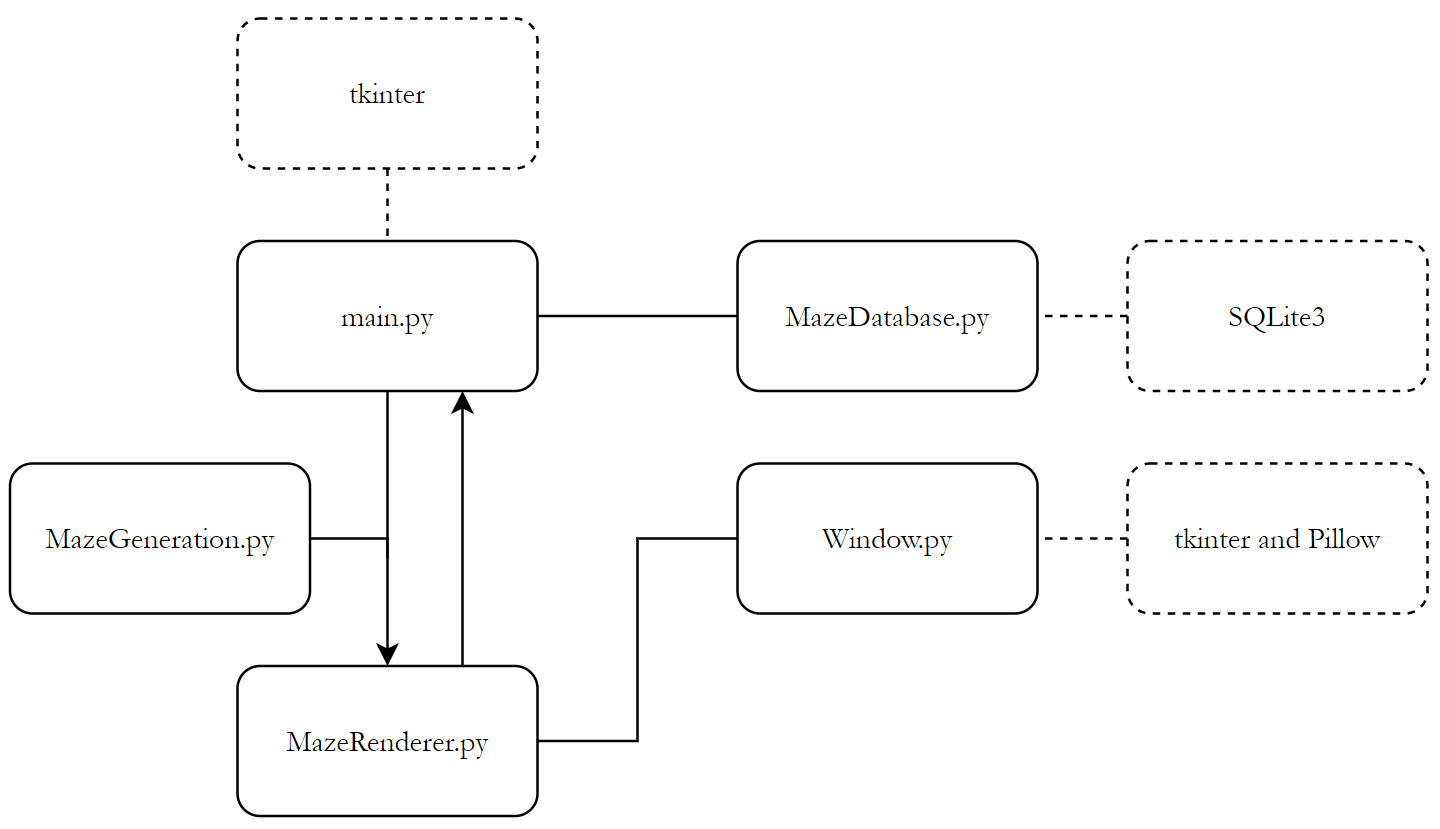
\includegraphics[scale=0.5]{Code Organization Diagram}}
%\end{center}
The project will be organized into five scripts, each handiling sections of the project;
\begin{itemize}
\item main.py - Controls/Passes data to the scripts, MazeDatabase, MazeGeneration and MazeRenderer aswell as handiling G.U.I.
\item MazeGeneration.py - Handles maze generations, returning maze\_data arrays that represent mazes.
\item MazeDatabase.py - Controls a user information and completed levels relational database, utilizing SQLite3.
\item Window.py - The previously discussed implementation of tkinter and Pillow to create rendering. It will also handle input attached to the windows it creates.
\item MazeRenderer.py - Handles game logic (such as collision) and implements the Window.py script to display the visuals on screen and control the player.
\end{itemize}

%%%%%%%%%%%%%%%%%%%%%%%%%%
\clearpage
\part{Documented Design}
\section{Program Organization Diagram}
\begin{center}
	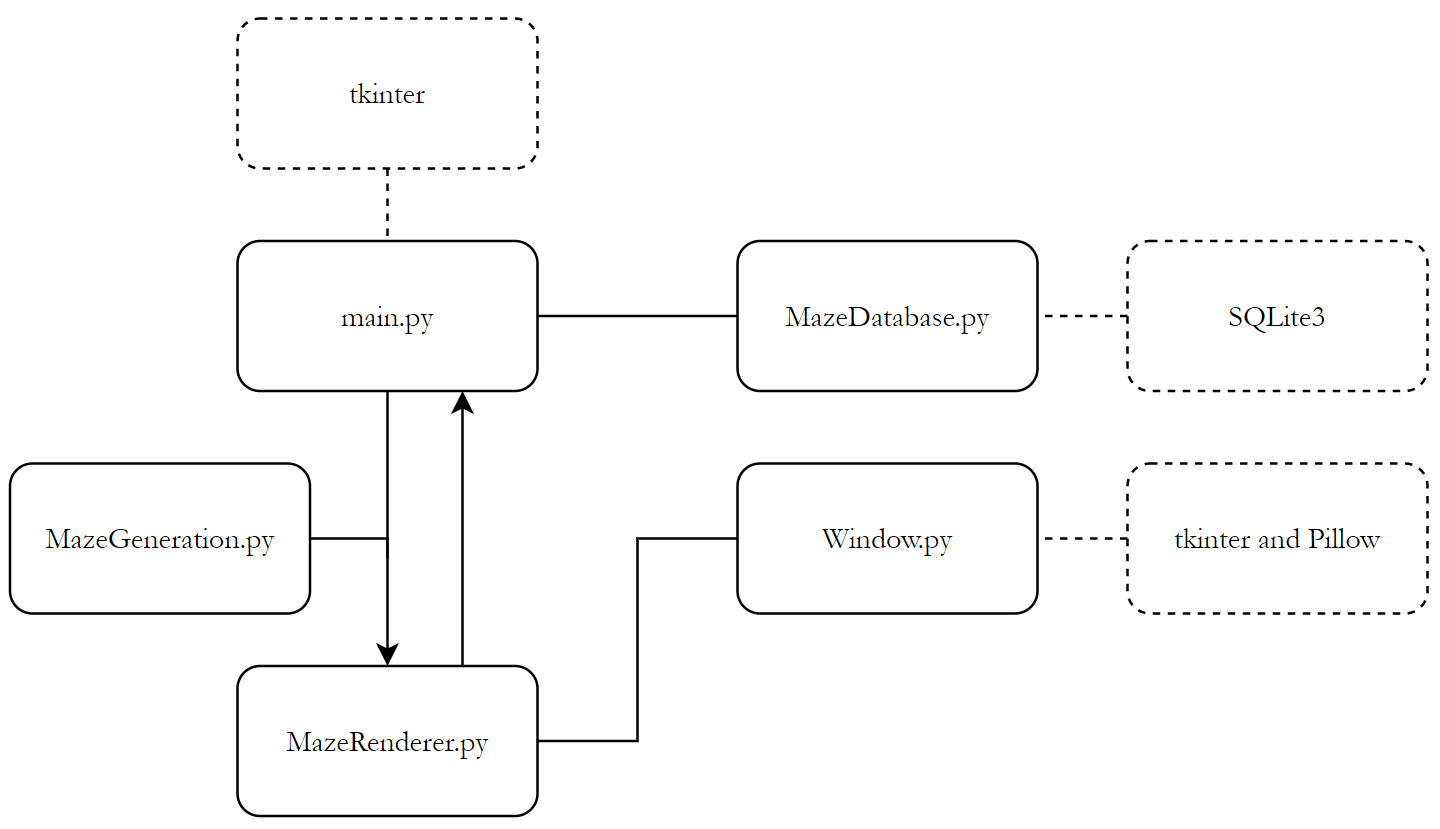
\includegraphics[scale=0.5]{Code Organization Diagram}
\end{center}
Above is a diagram showcasing all the scripts listed in the Organization of Solution section. "main.py" is the starting point, which will also communicate with "MazeDatabase.py"
to handle users/saving completed levels. It also has a link to tkinter, though in the diagram the link is dotted as while tkinter is vital to "main.py" script it is not code I have written.
This is the same relationship with "MazeDatabase.py" and SQLite3. The final link is to "MazeRenderer.py", however, the link itself is connected to "MazeGeneration.py" this is because
while "MazeGeneration.py" is controlled by "main.py" the generated maze is immediately passed to "MazeRenderer.py".
"MazeRenderer.py" has a link to "Window.py" which it uses to create the window of editable pixels used to render the game. There is also a link back to "main.py" as the user
is returned there after the level is completed or quit. "Window.py" also has a dotted link to tkinter and Pillow for the same reason as "main.py" and "MazeDatabase.py" mentioned above.
\clearpage
\section{Window/Layer Class Diagrams}
\begin{center}
	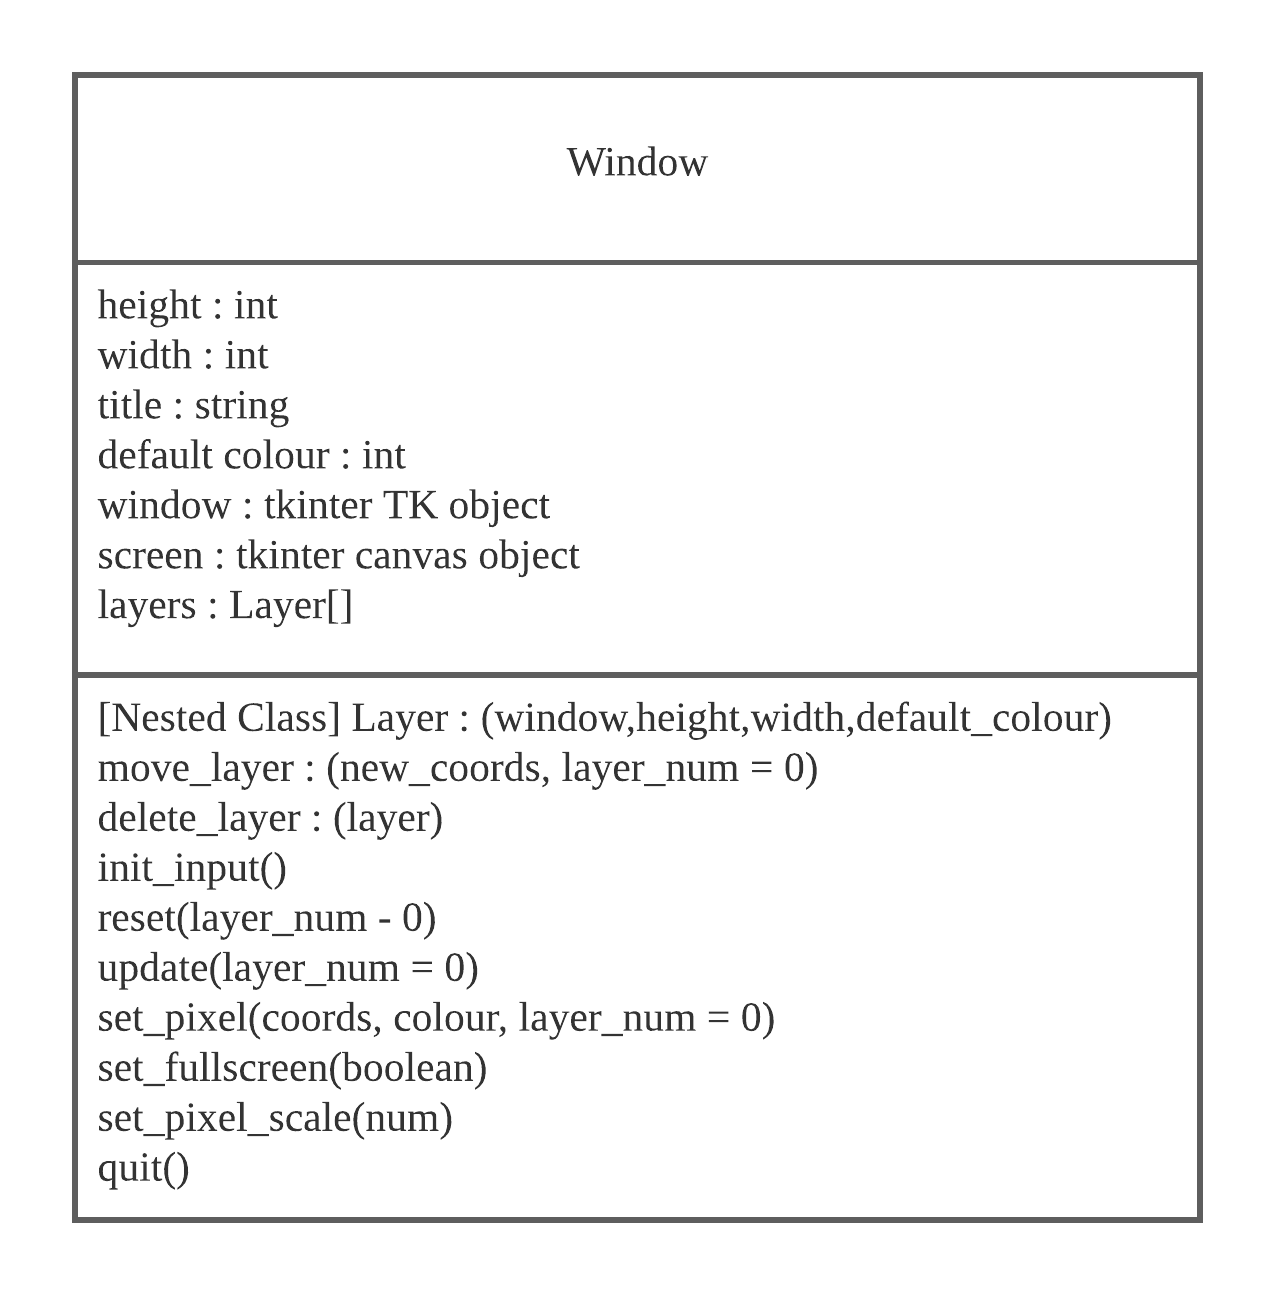
\includegraphics[scale=1]{Window Class}
	%Should probably colour code the above diagram at some point
\end{center}
\begin{center}
	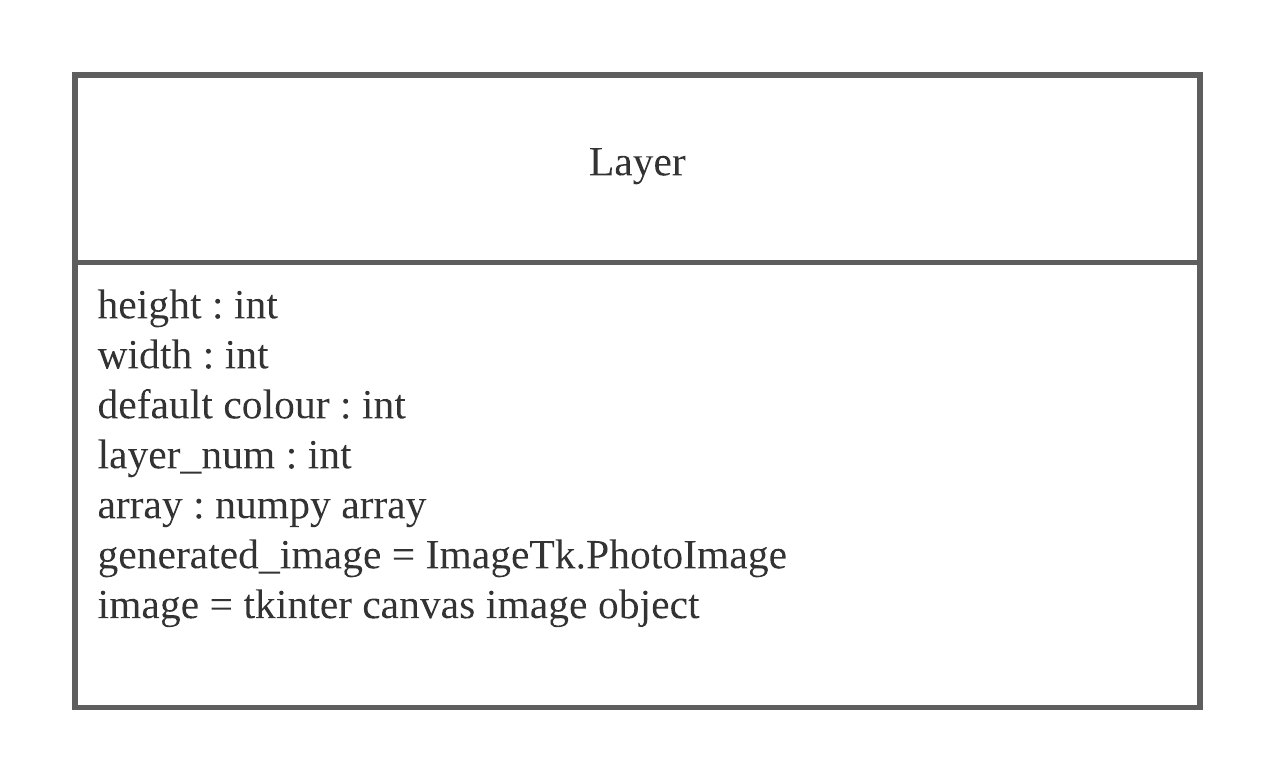
\includegraphics[scale=1]{Layer Class}
	%Should probably colour code the above diagram at some point

	\color{mygrey}(Note: In Python a nested class doesn't imply any relationship)
\end{center}

\clearpage
\section{Maze Select G.U.I}
\begin{center}
%Start Screen
	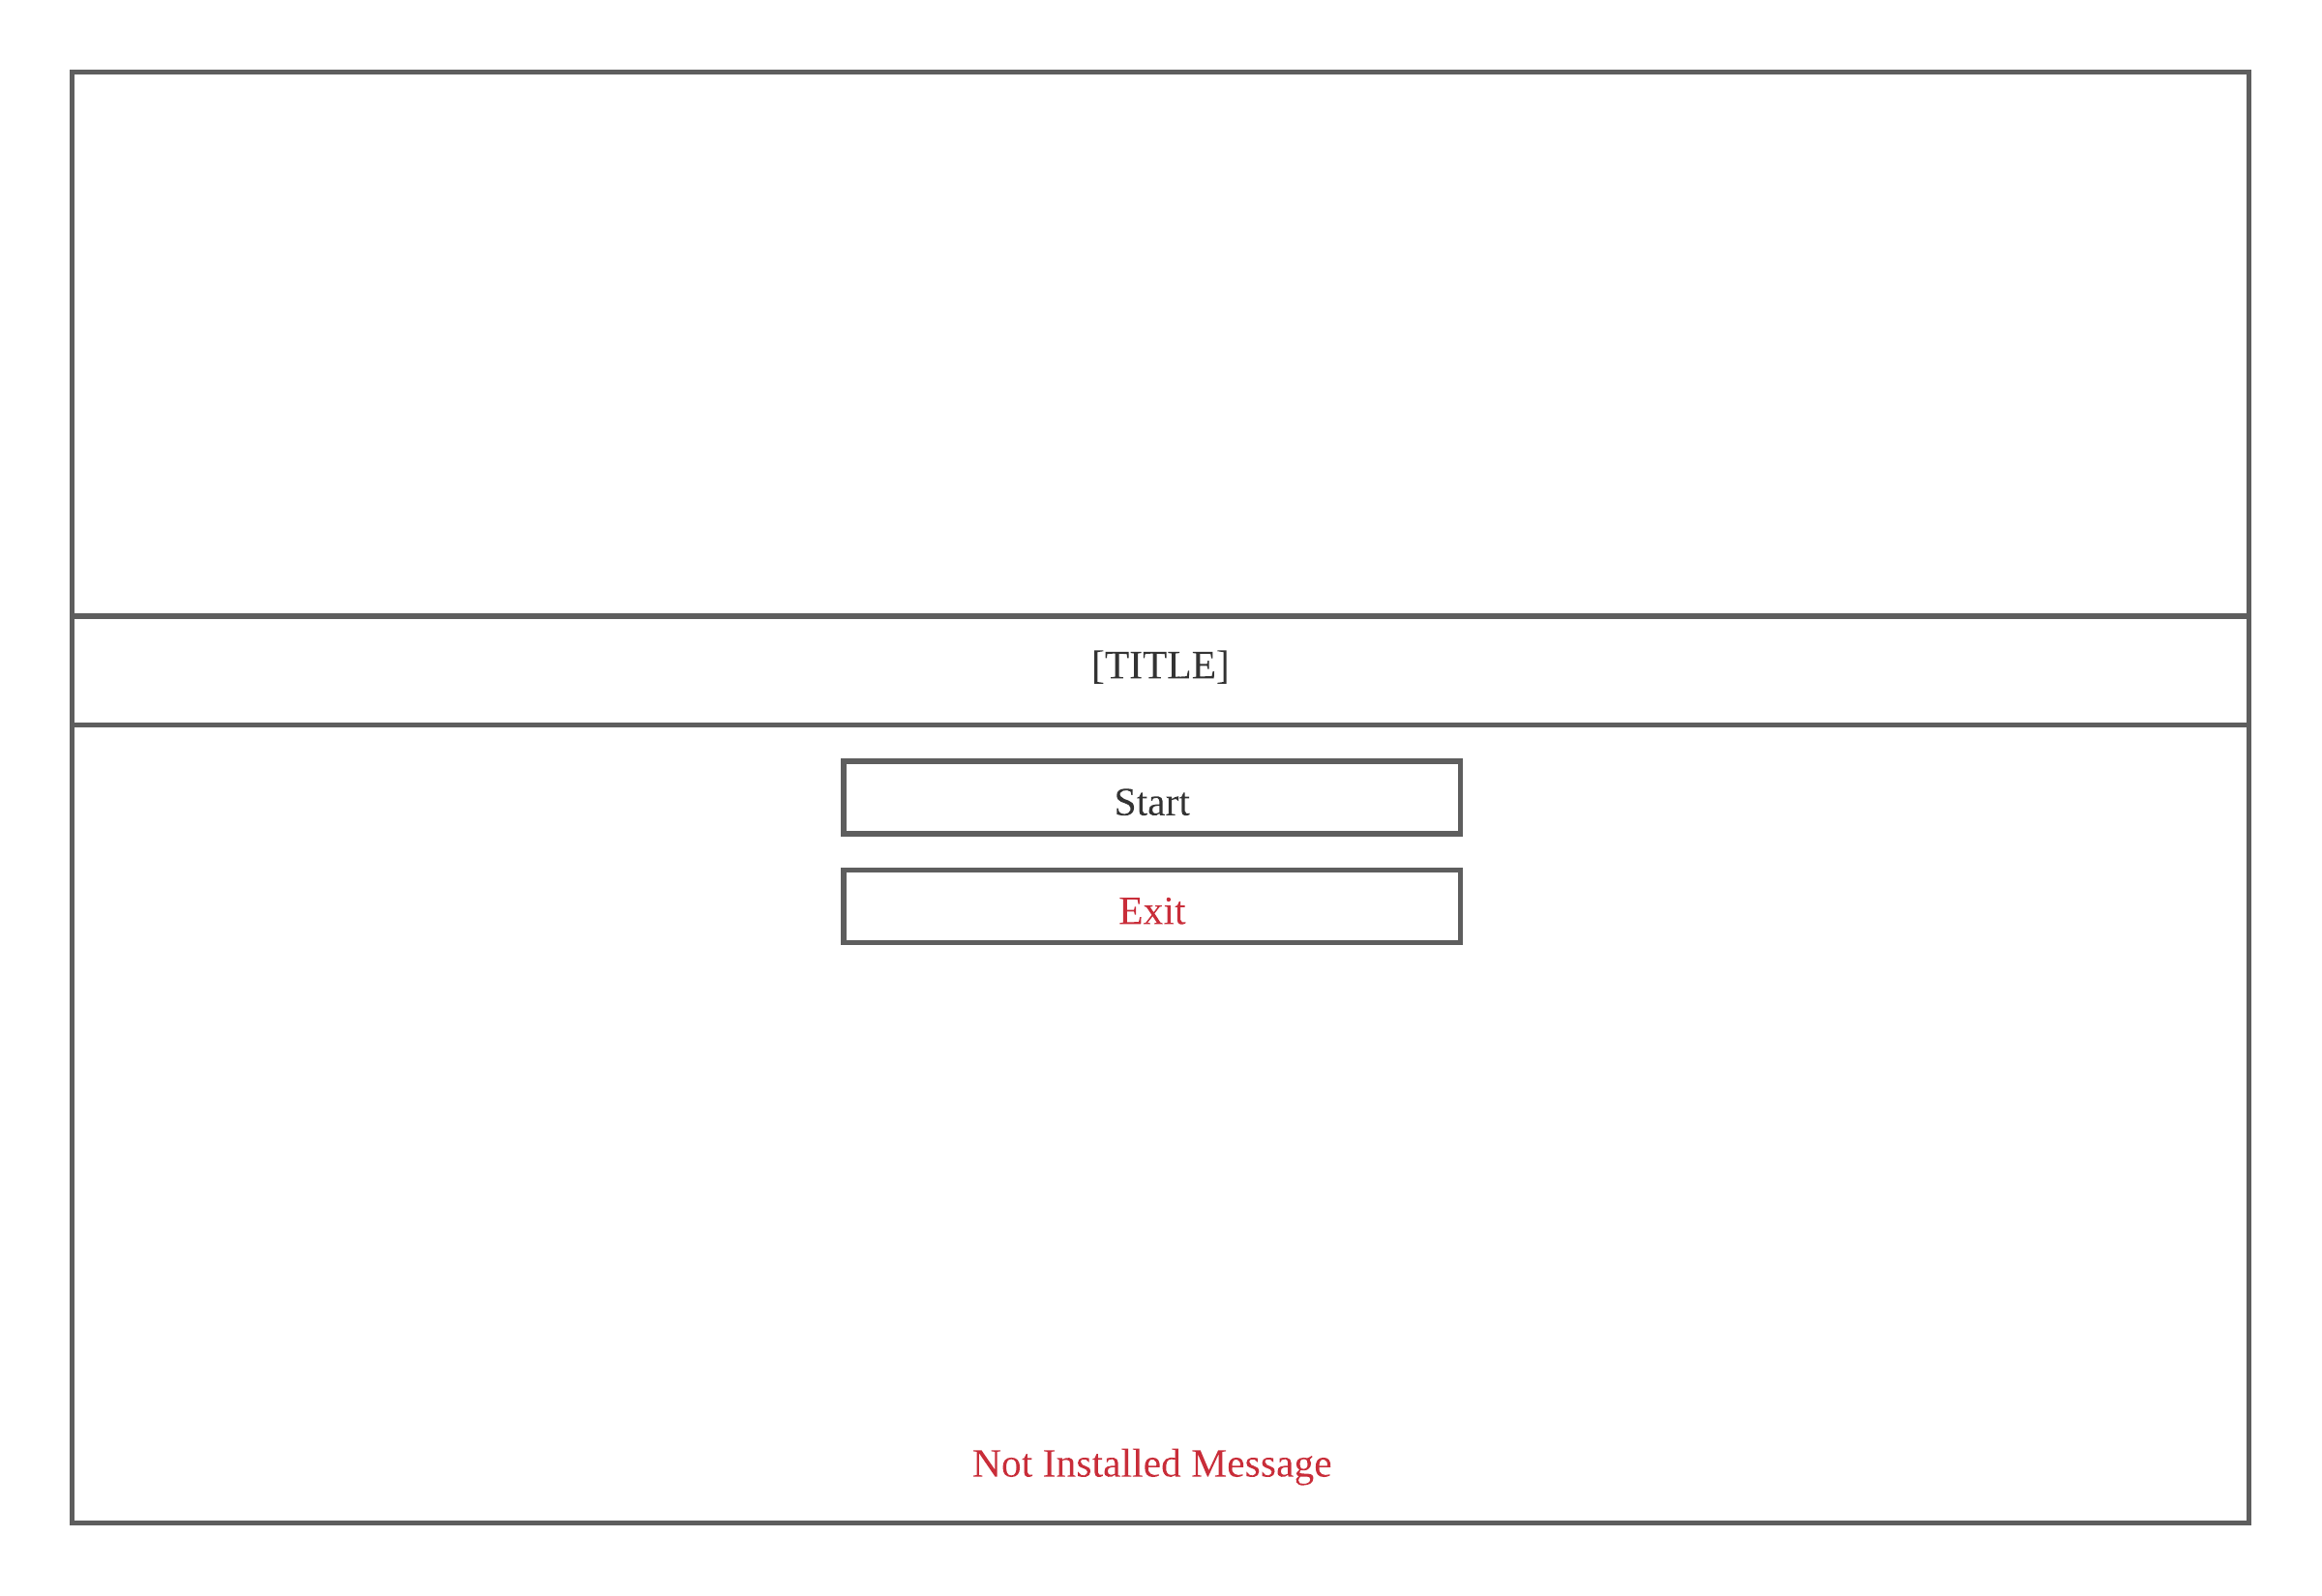
\includegraphics[scale=0.7]{Start Screen}

	Above is the start screen, it features the title and two buttons. The first button is the start button which will lead to the user select
	screen and the second is the exit button which will simply close the button.
\end{center}
\begin{center}
%User Select Screen
	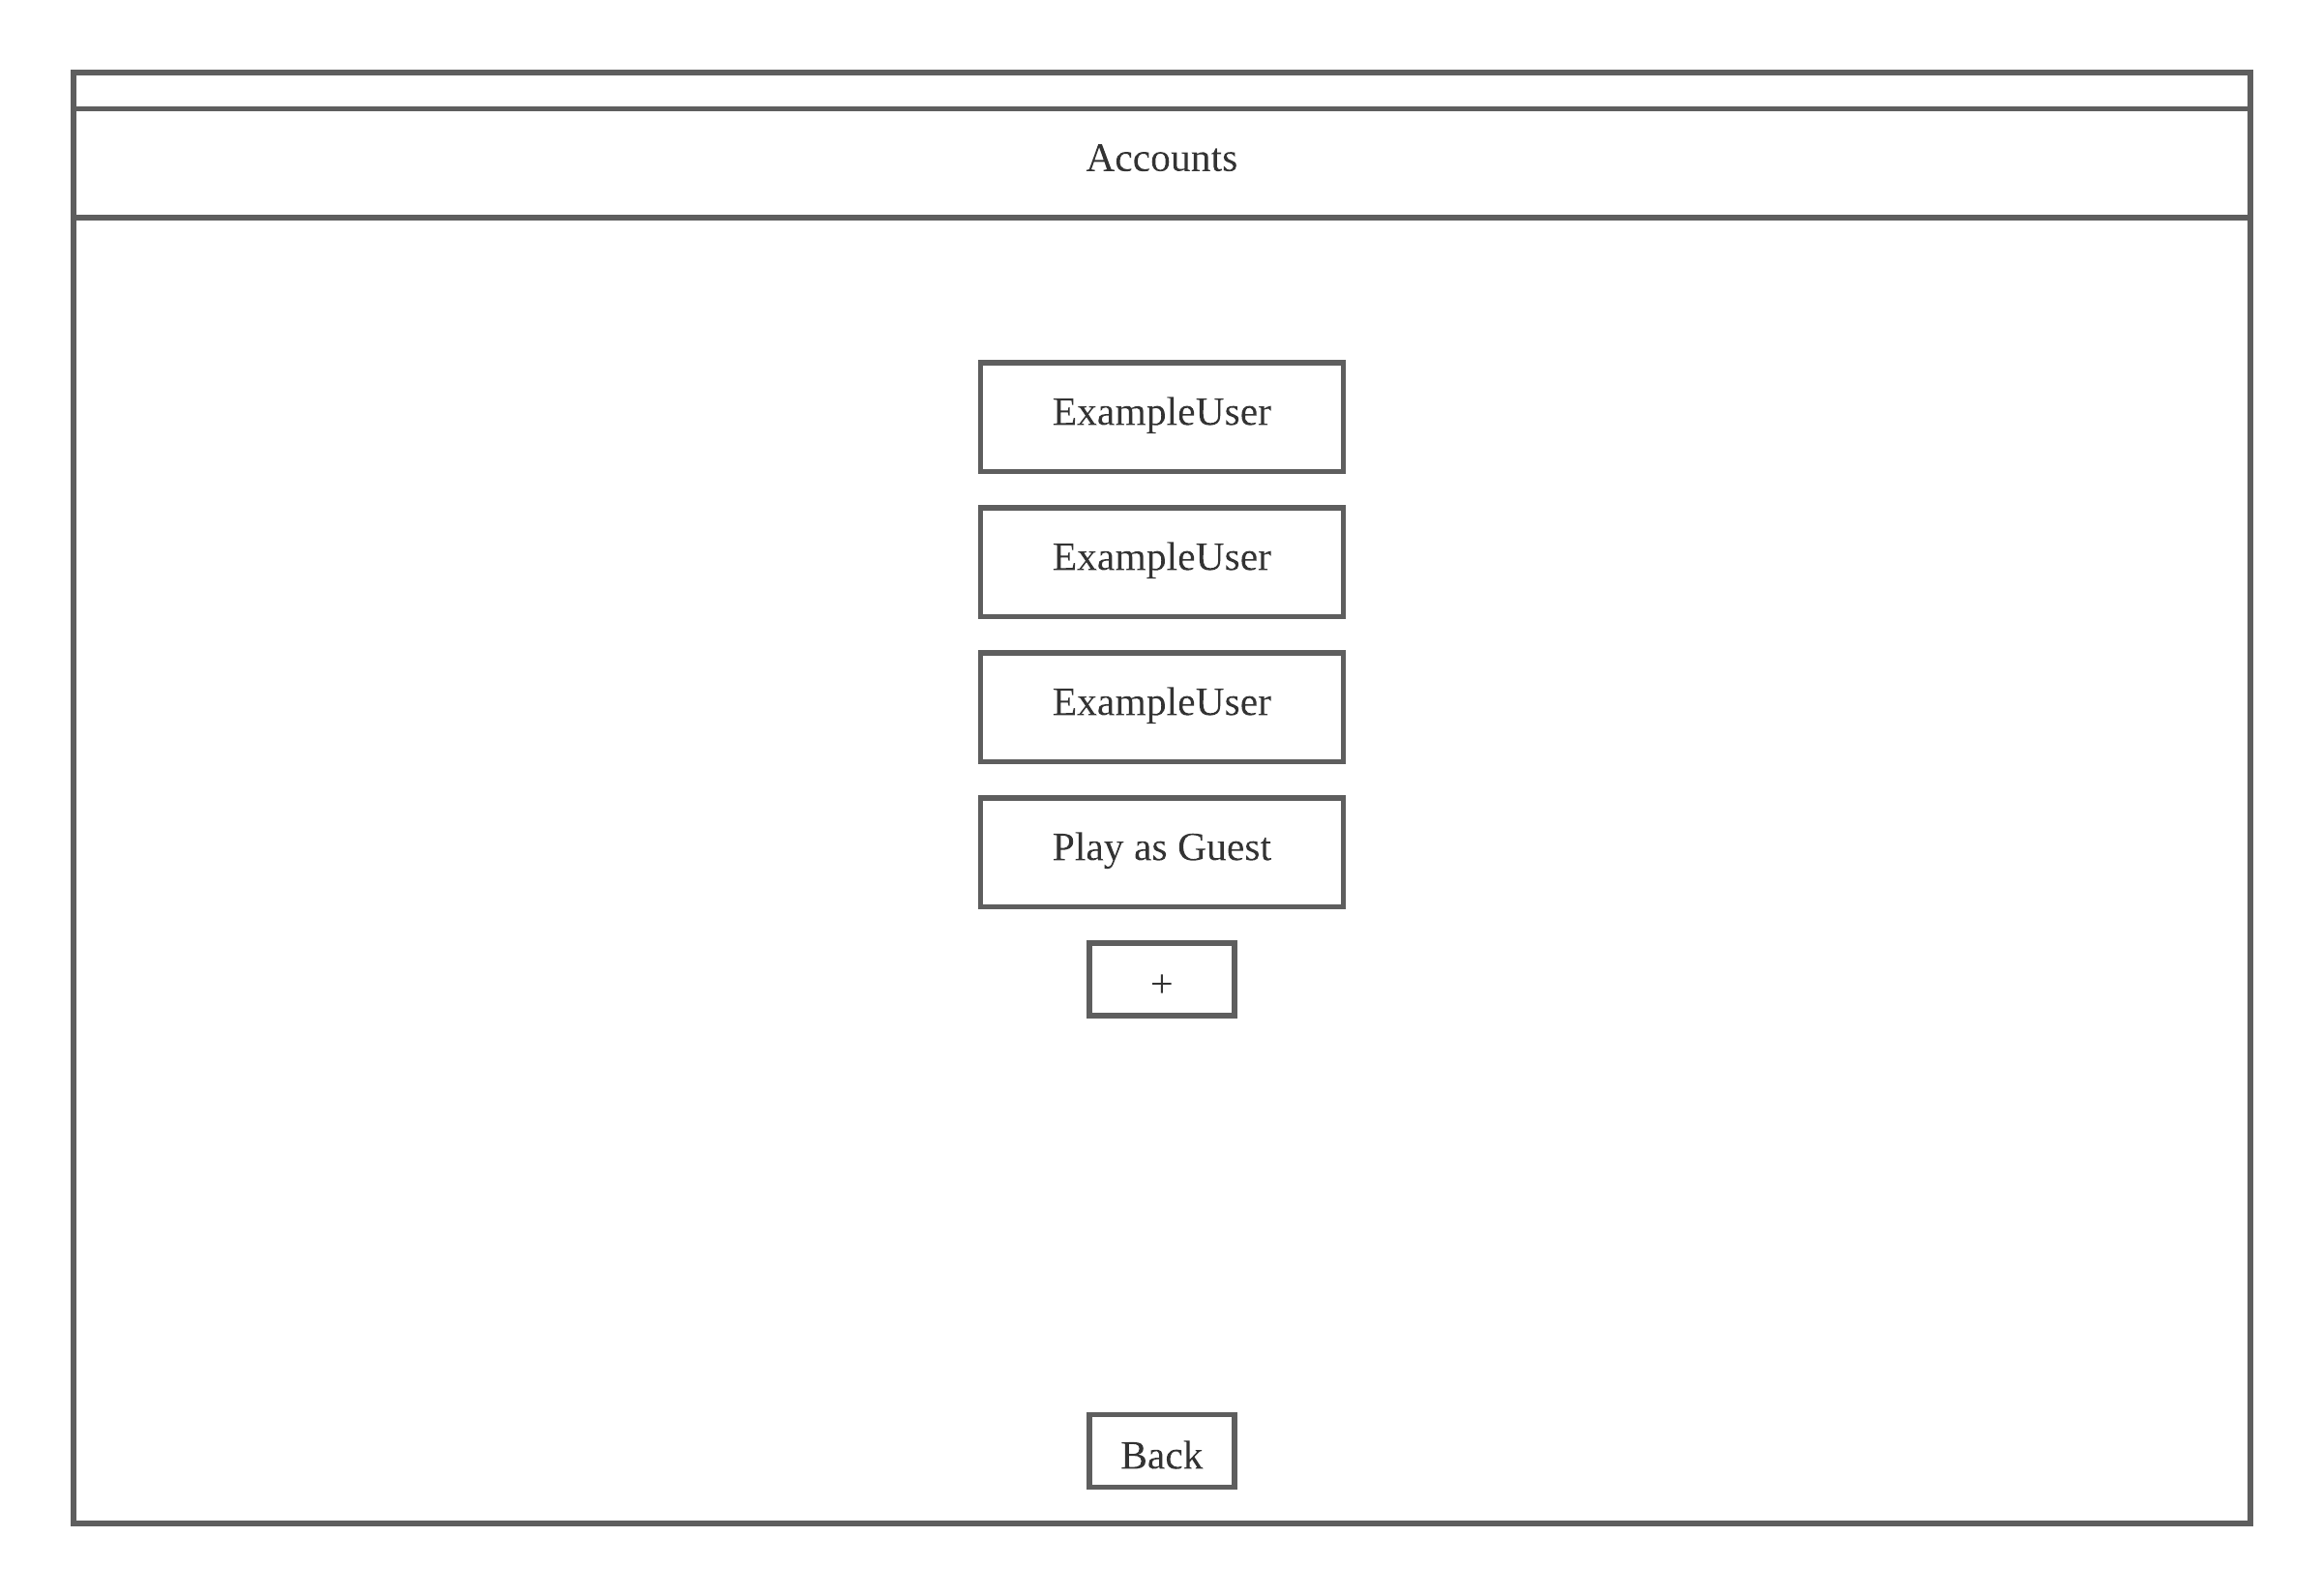
\includegraphics[scale=0.7]{User Select Screen}

	On the user select screen there is a list of created users, a play as guest button, a button to add a new user (the plus) and a back button. The back button
	will send that user back to the start screen.
\end{center}

\begin{center}
%New User Screen
	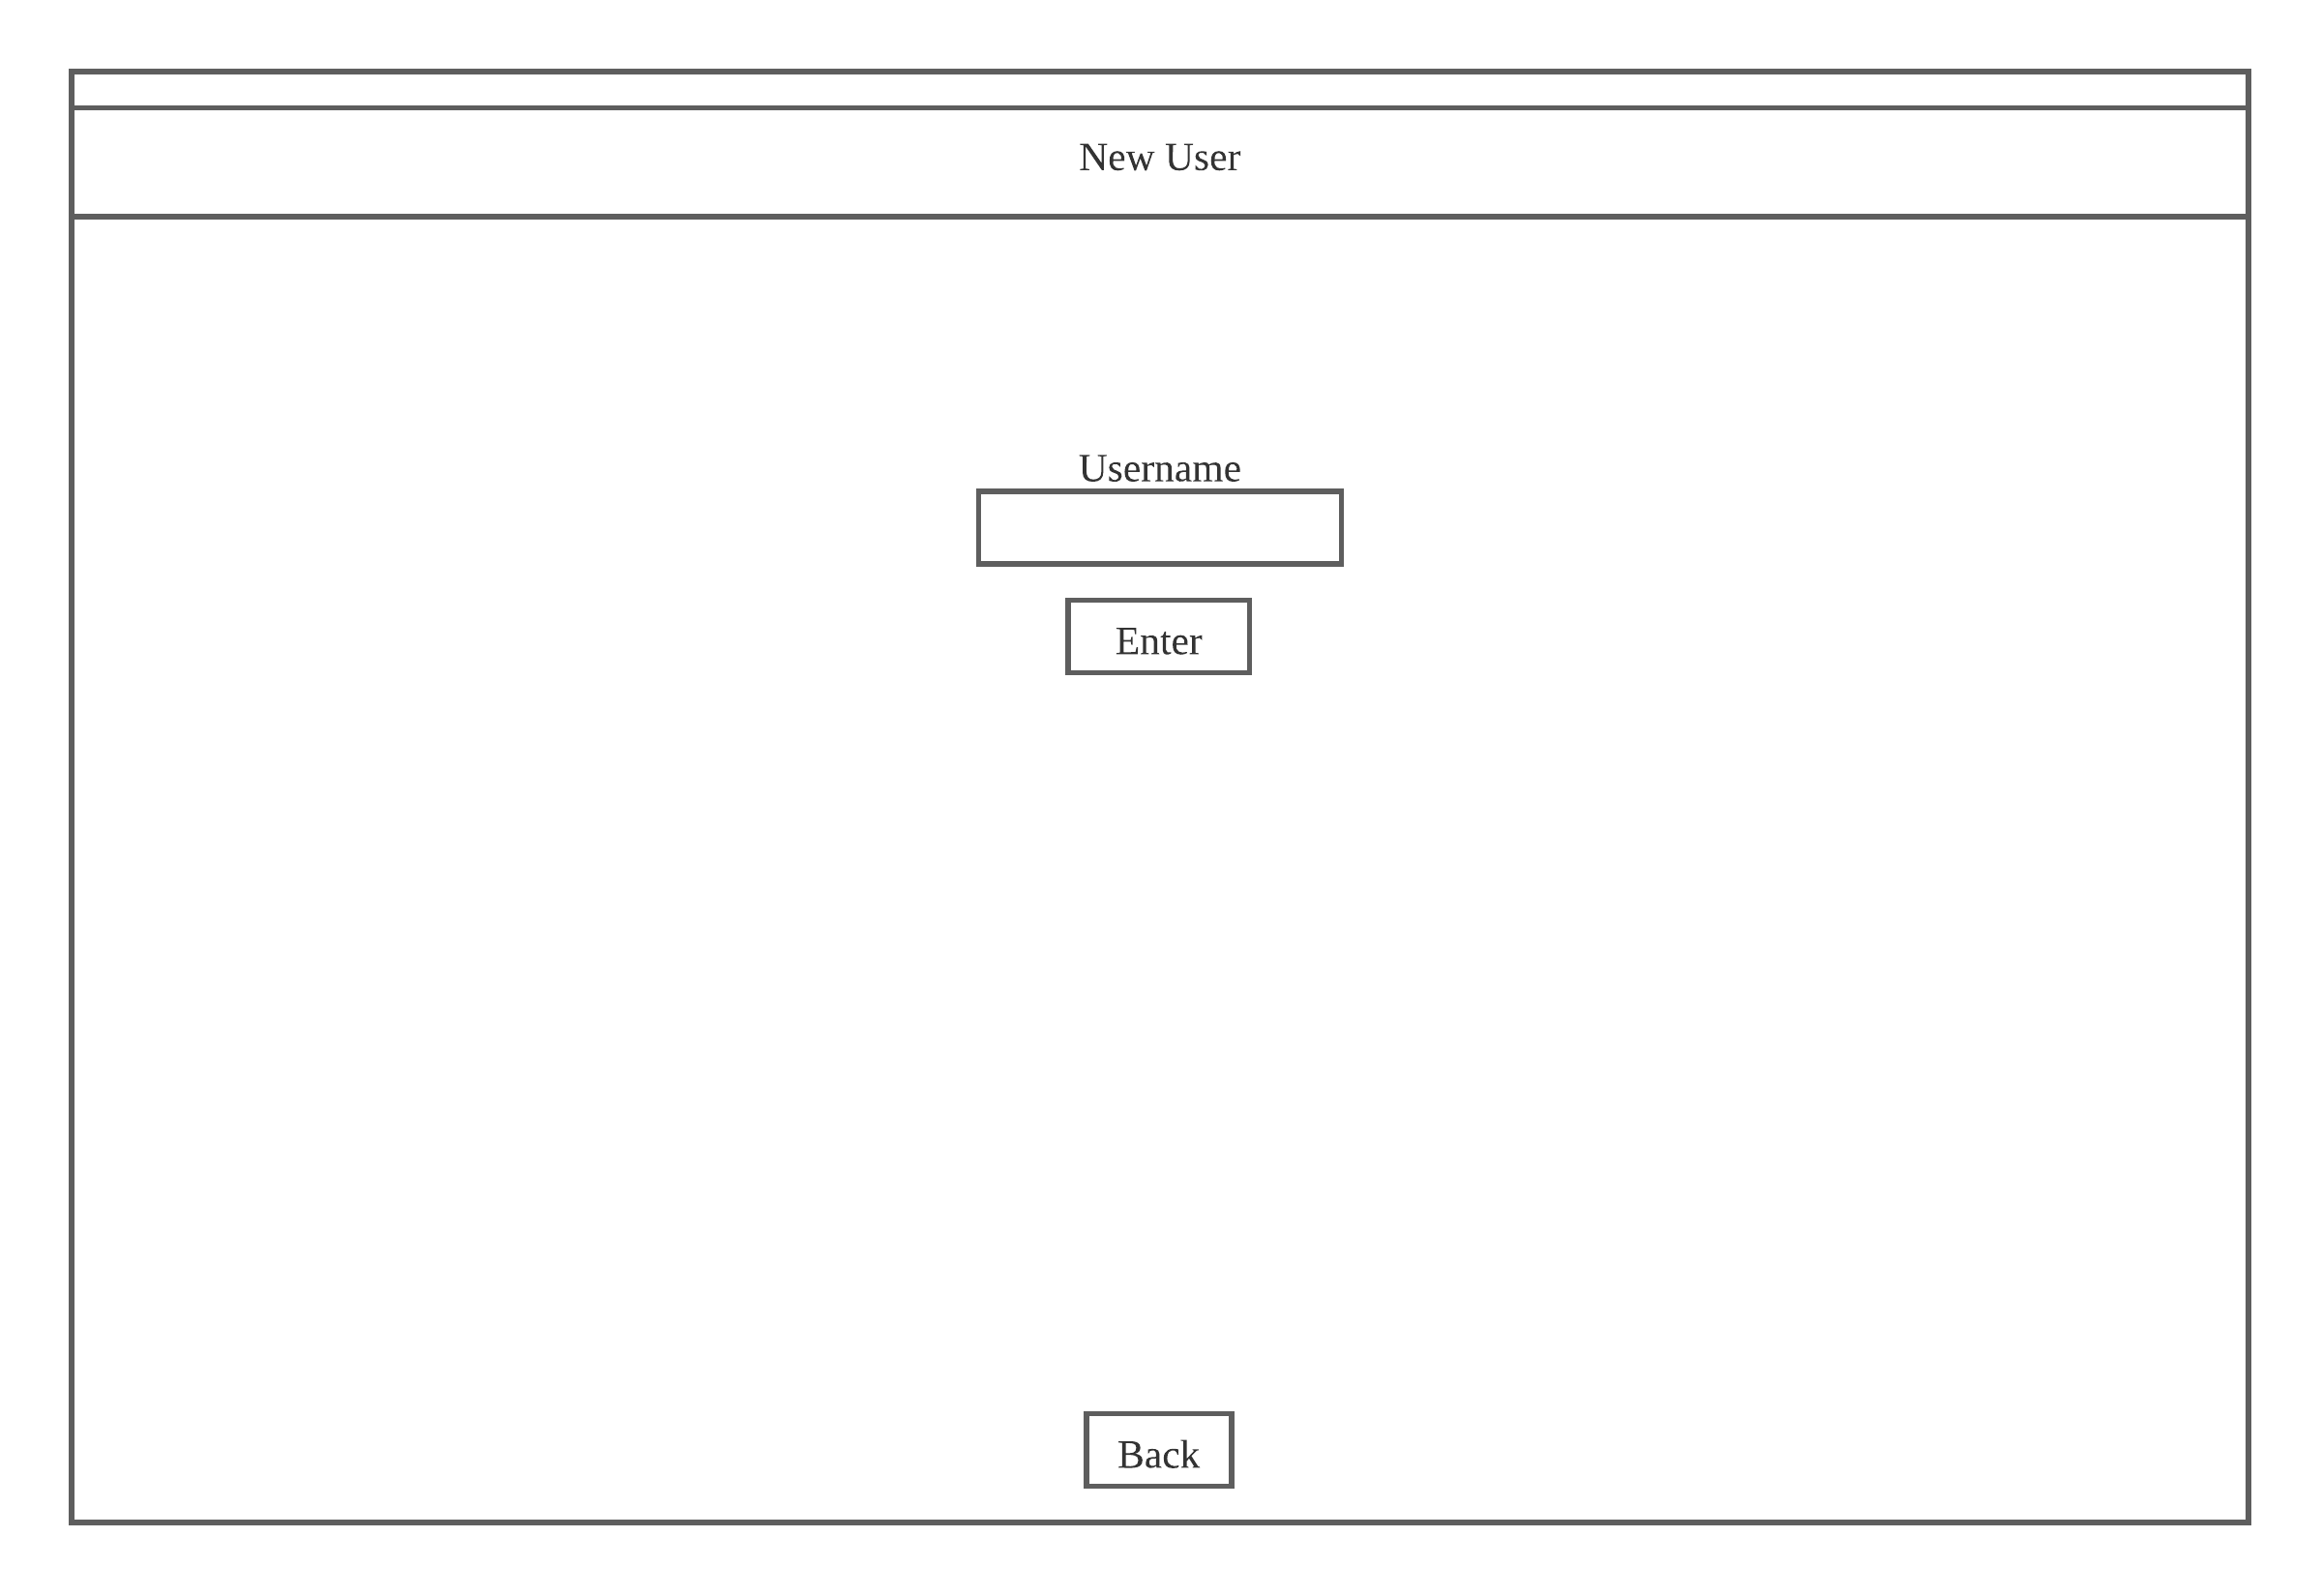
\includegraphics[scale=0.7]{New User Screen}

	The new user screen only needs to include an entry bar for the name to be typed in, a button to confirm the username and a back button (to take the user back to the
	user select screen). There is exception handiling to stop a username being entered that is blank.
\end{center}

\begin{center}
%Maze type Select Screen
	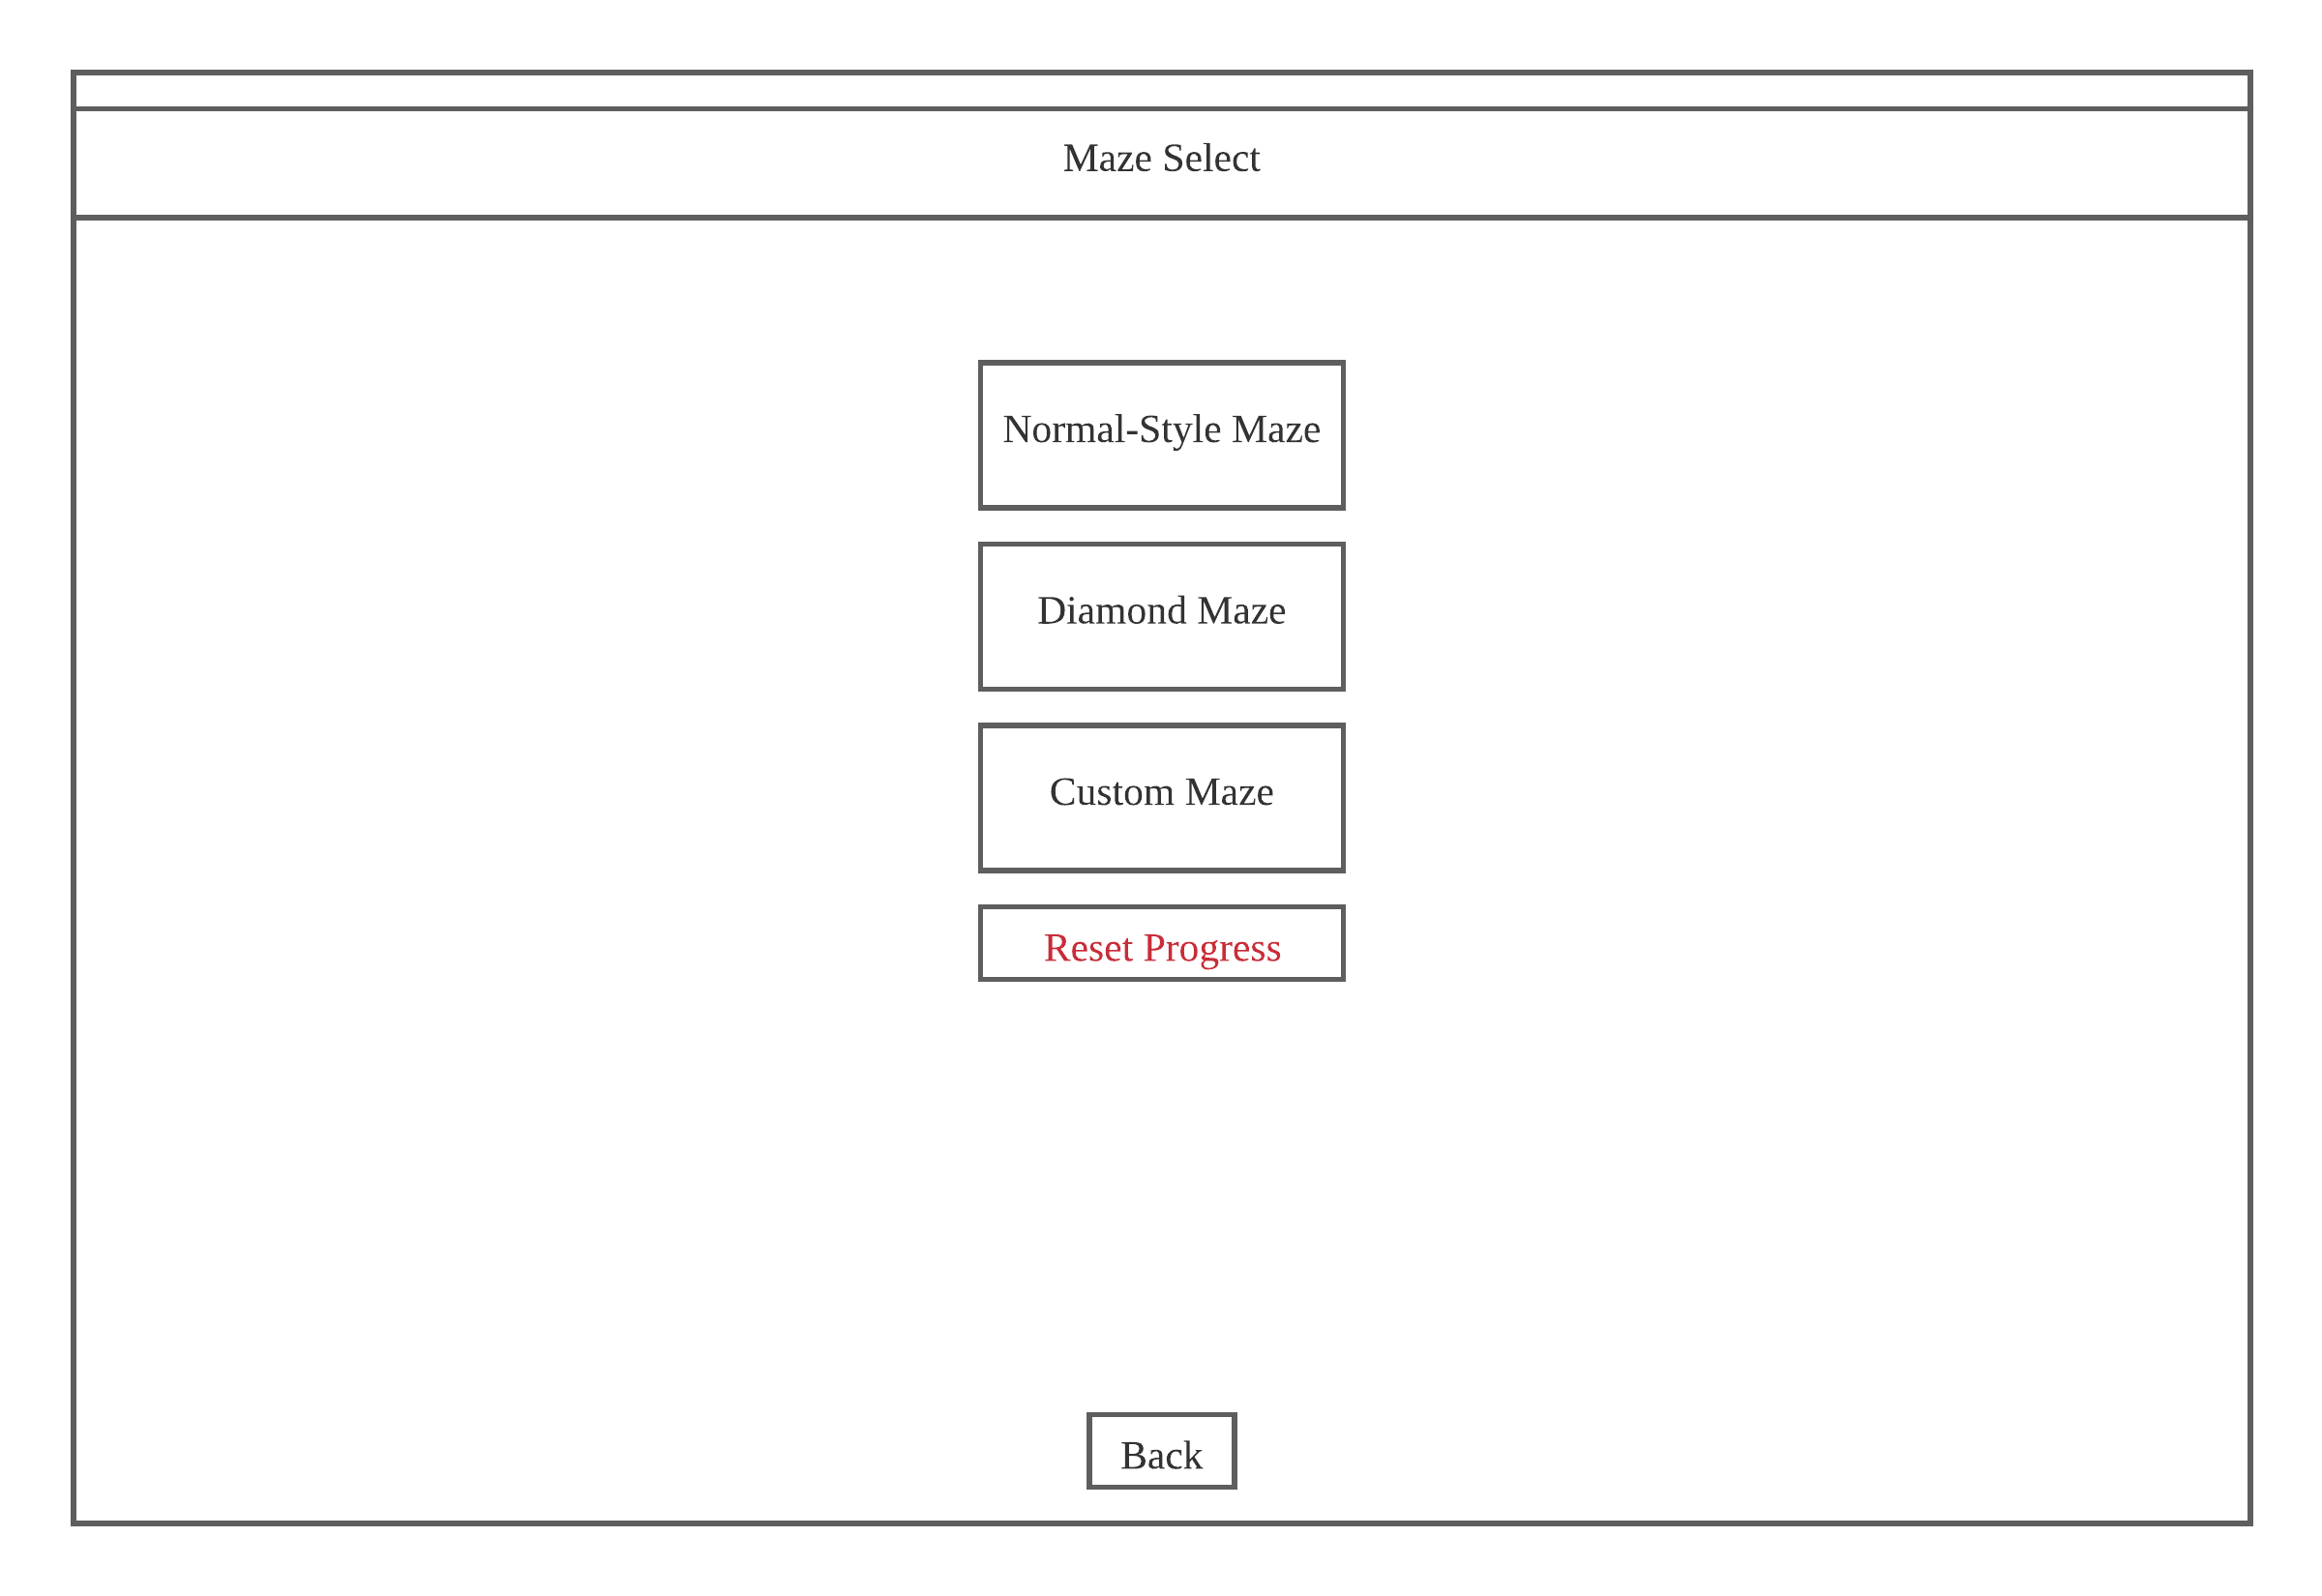
\includegraphics[scale=0.7]{Maze Select Screen}

	On the maze select screen all current maze types are displayed as buttons, in the image above these are; "Normal-Style Maze", "Diamond Maze" and "Custom Maze".
	There is also a "Reset Progress" button that, if the user isn't a guest, will reset their completed levels entry in the maze database. It also has a back button which takes
	the user back to the user select screen.
\end{center}

\clearpage
\begin{center}
%Level Select Screen
	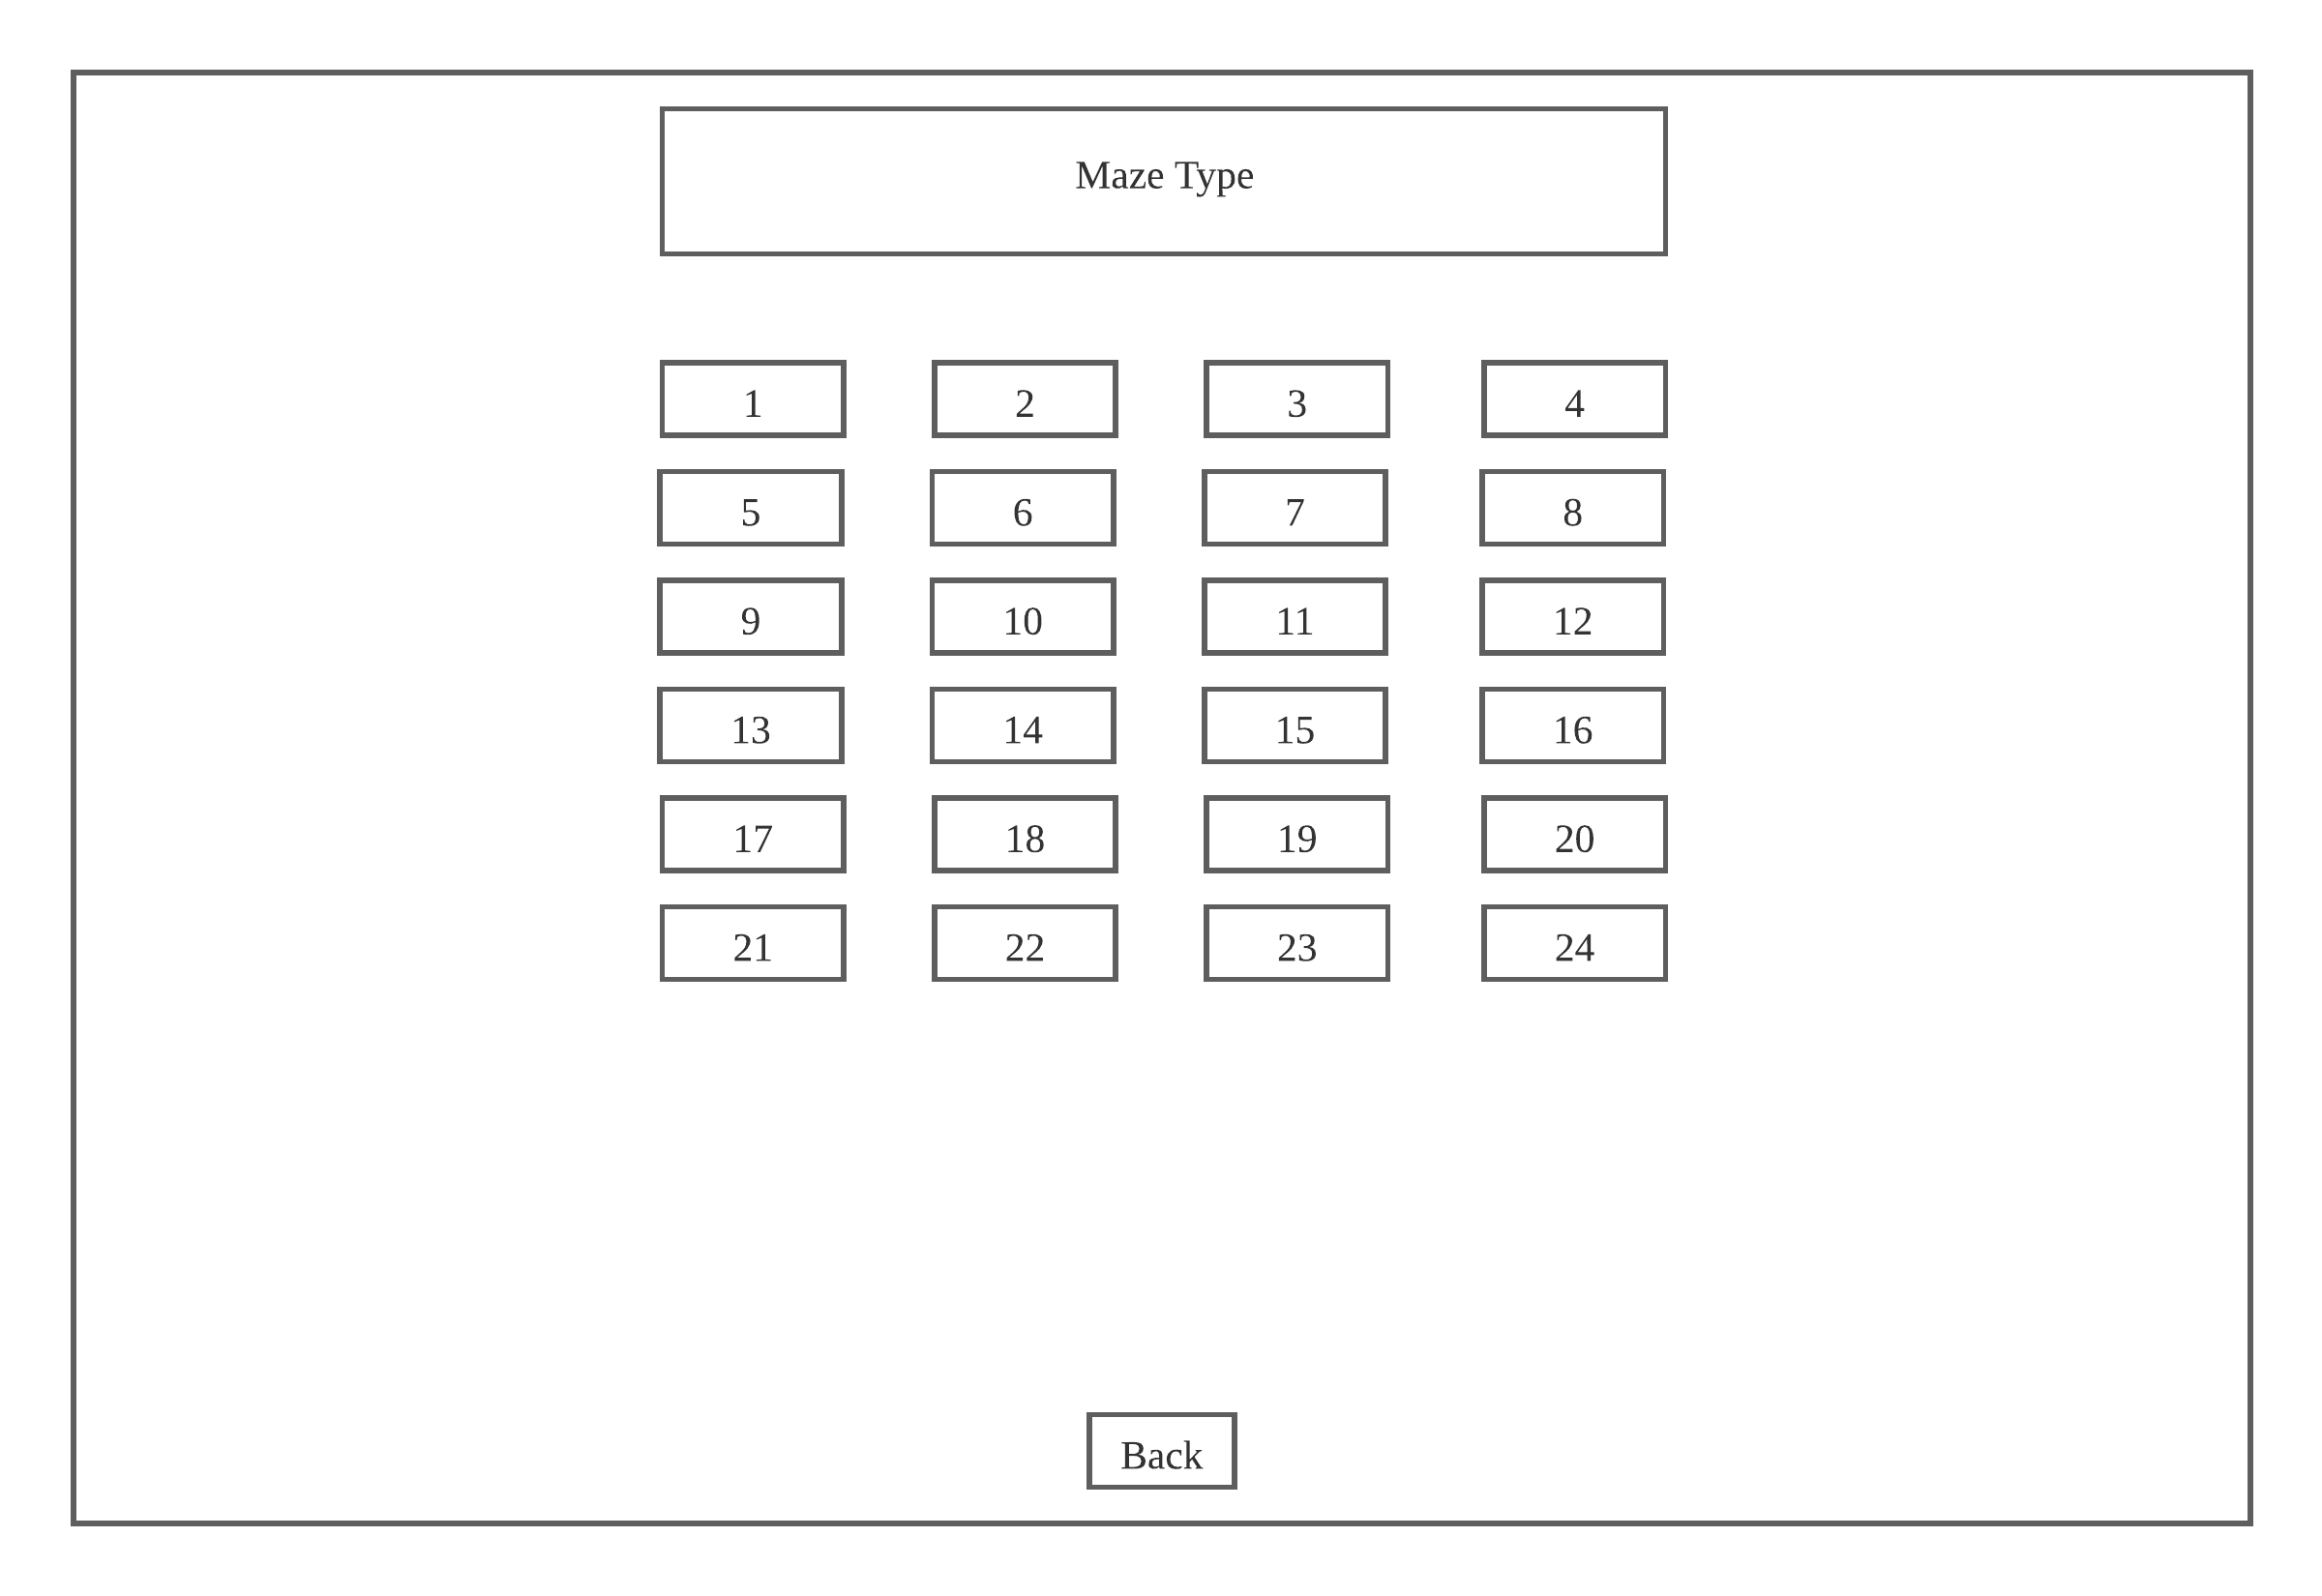
\includegraphics[scale=0.7]{Maze Level Select}

	The maze level select screen consists of rows of buttons that are generated iteratively, each button with a number correlating to the difficulty of the level
	(The actual size of the maze is the number+3). Like the other screens there is a back button, which in this case, leads back to the maze type select screen.
\end{center}
\begin{center}
%Custom Maze Screen
	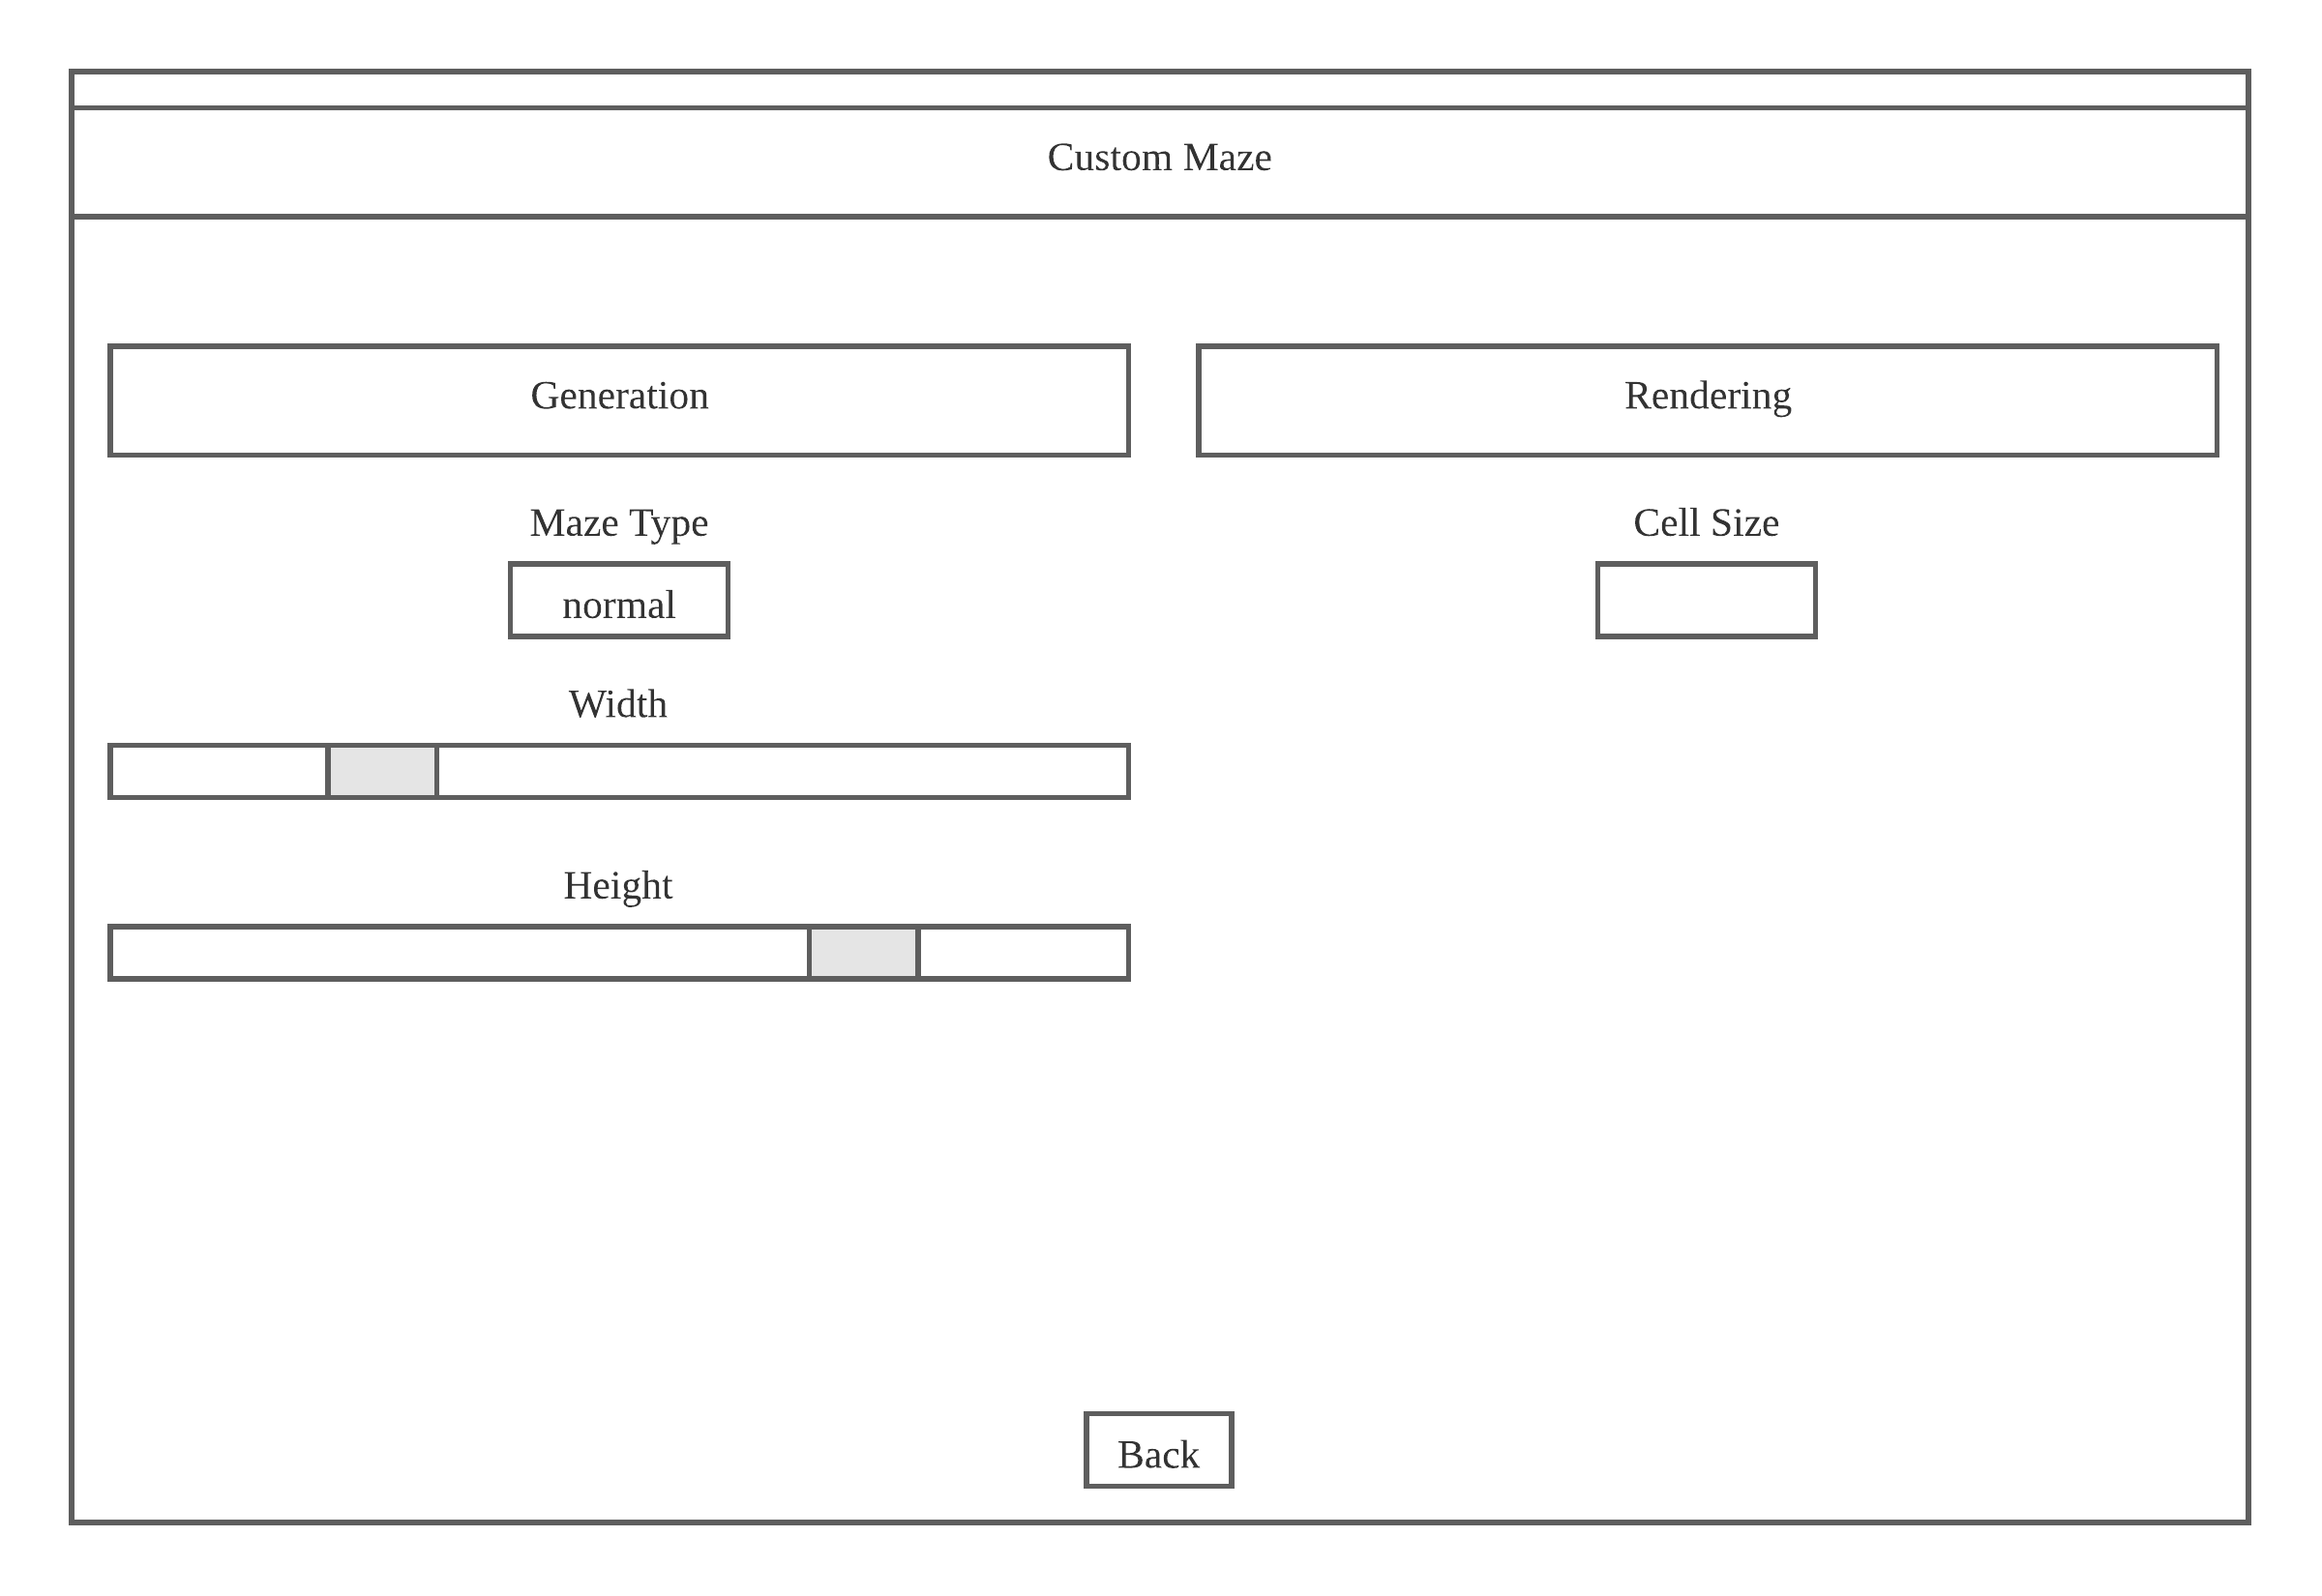
\includegraphics[scale=0.7]{Custom Maze Screen}

	Included on the custom maze screen is halves, one dedicated to rendering and the other to generation. The generation options are maze type, width
	and height, while the only option for rendering is cell size. More options could certainly be added (as my rendering scripts allow for it) if I had more time.
\end{center}
\clearpage
\section{Game Visuals}
\begin{center}
%Loading Screen
	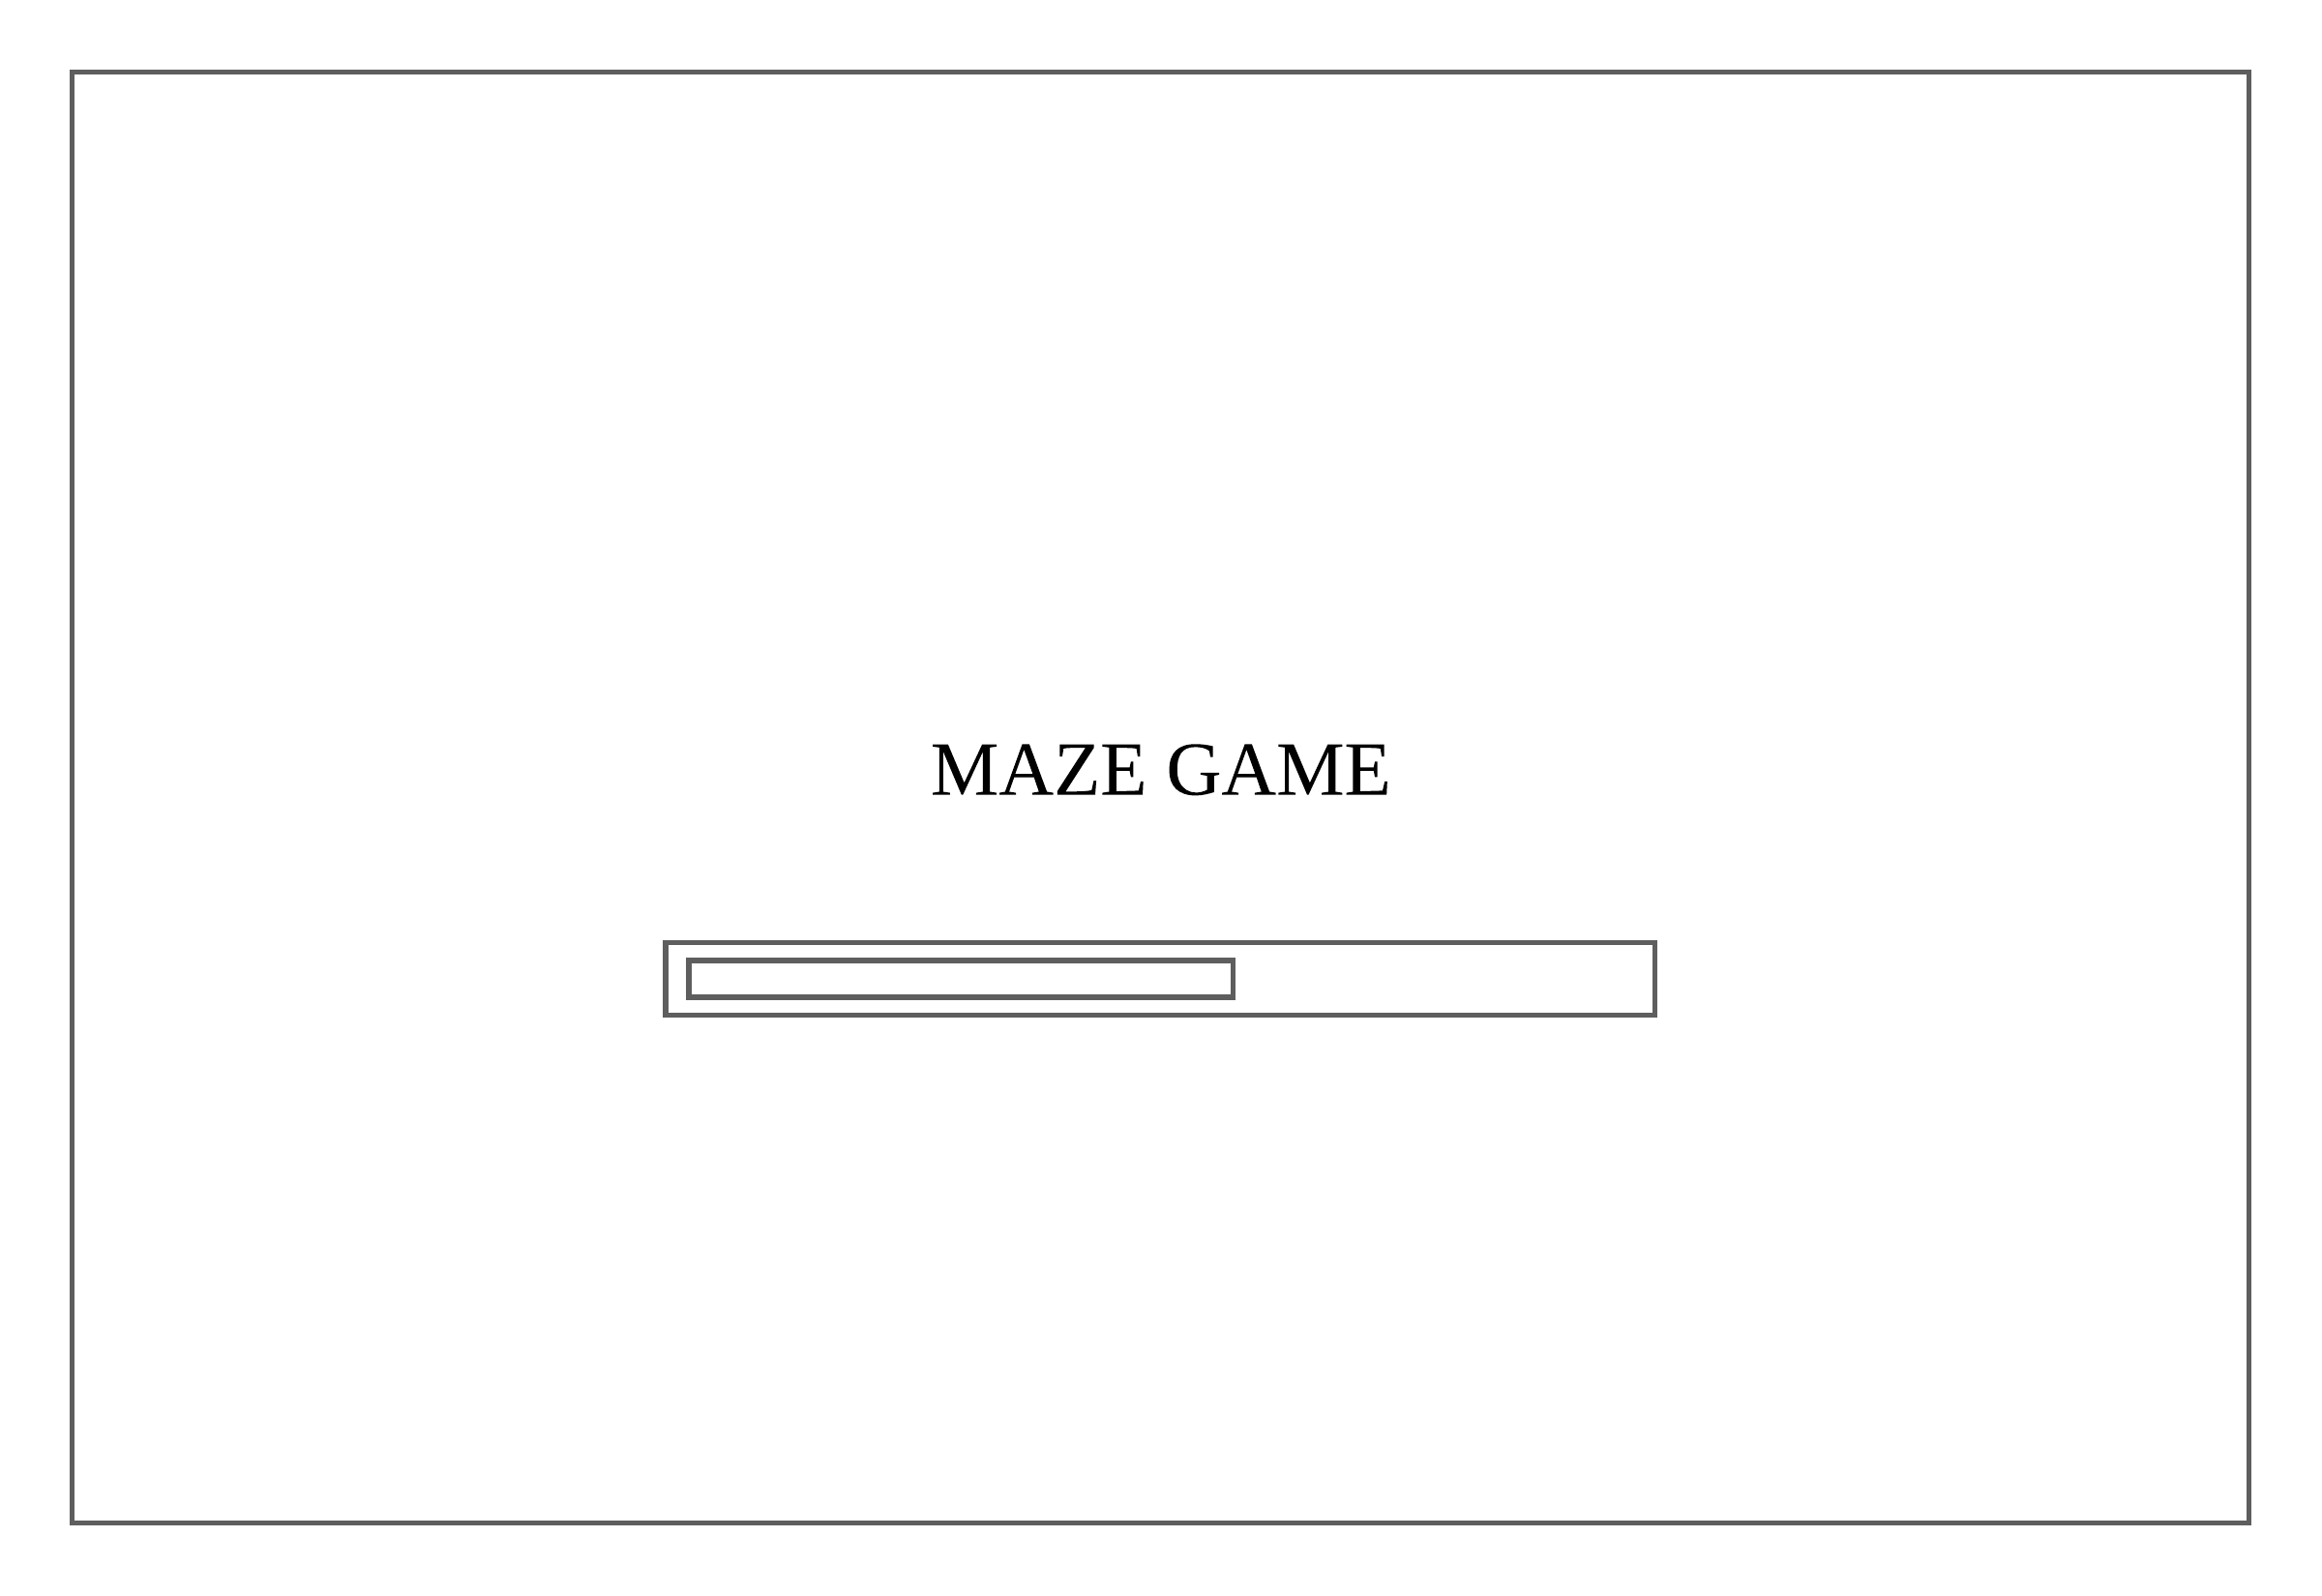
\includegraphics[scale=0.7]{Loading Screen}
	
	Above is the loading/title screen meant to create a slight delay between the level select screen and playing the actual maze, mainly to give the game
	a nicer feel. In actuality the loading bar isn't actual linked to any loading, though if I had more time, through the use of a recursive function, I could pair it with
	the maze generation.
\end{center}
\begin{center}
%Maze Screen
	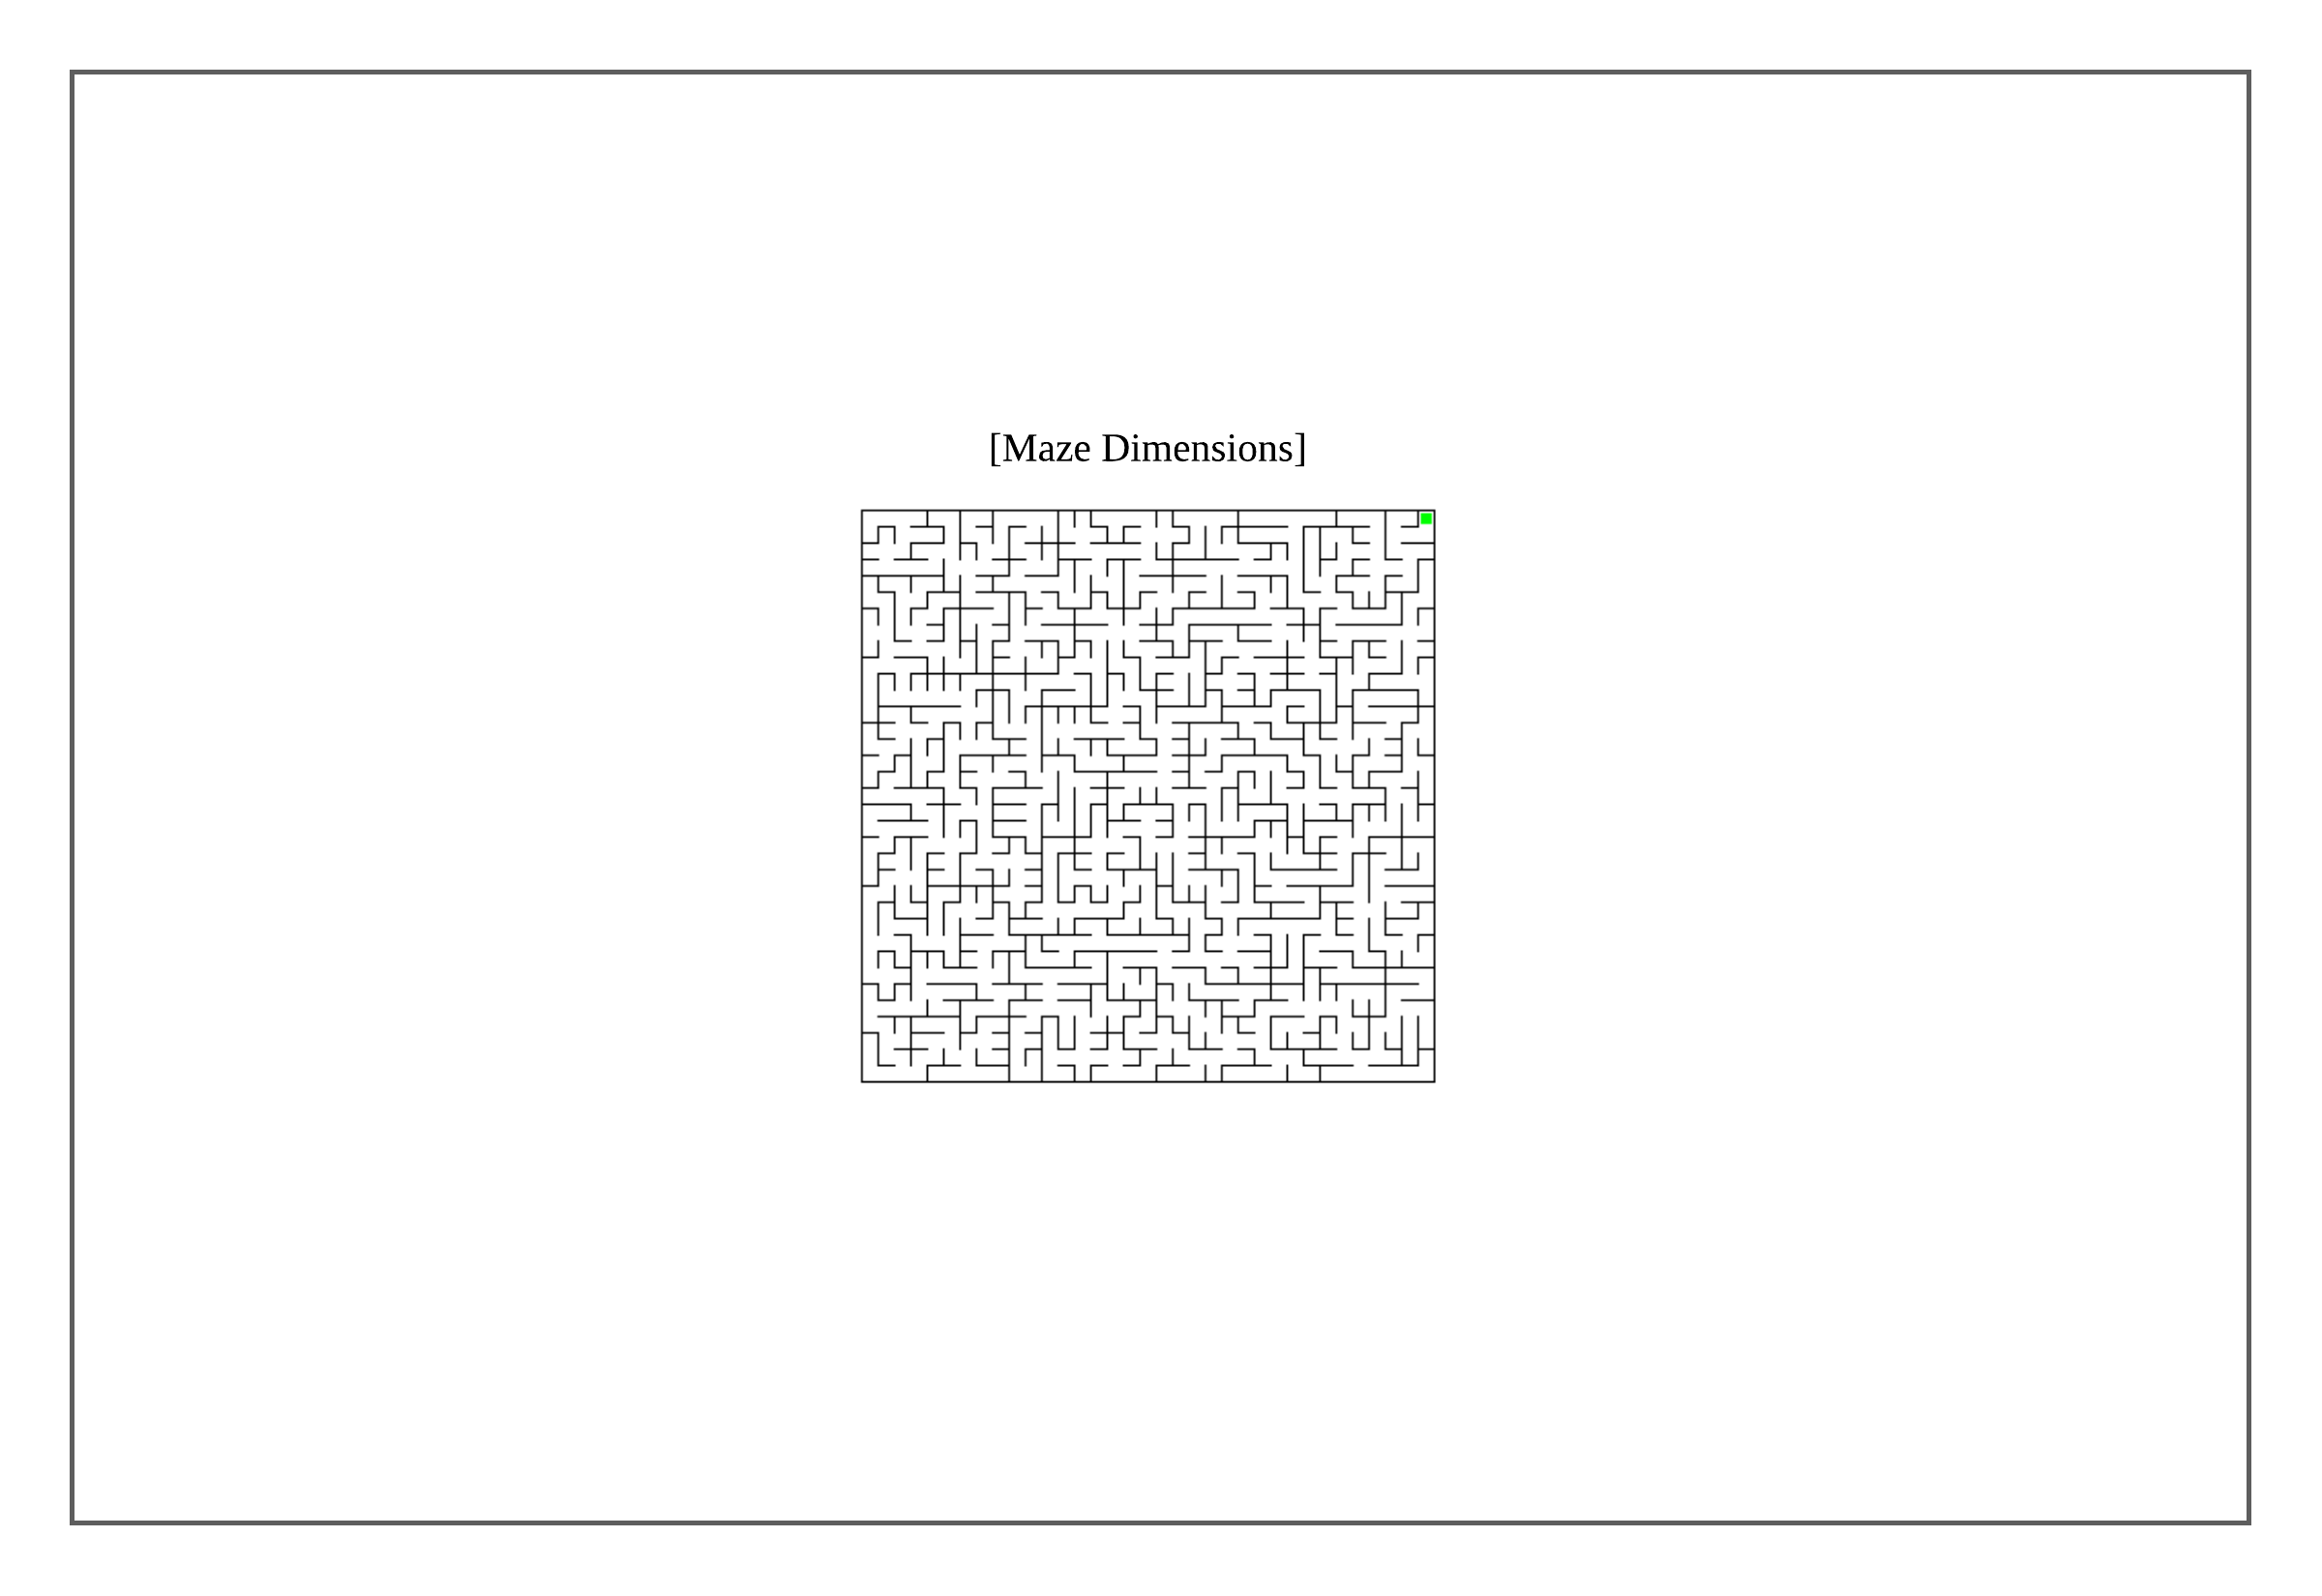
\includegraphics[scale=0.7]{Maze Screen}

	The screen above is where the actual maze will be played, with an example 35 by 35 maze shown.  Above the maze proper is the maze dimensions,
	serving as a title.
\end{center}
\clearpage
\begin{center}
%Maze Completed Screen
	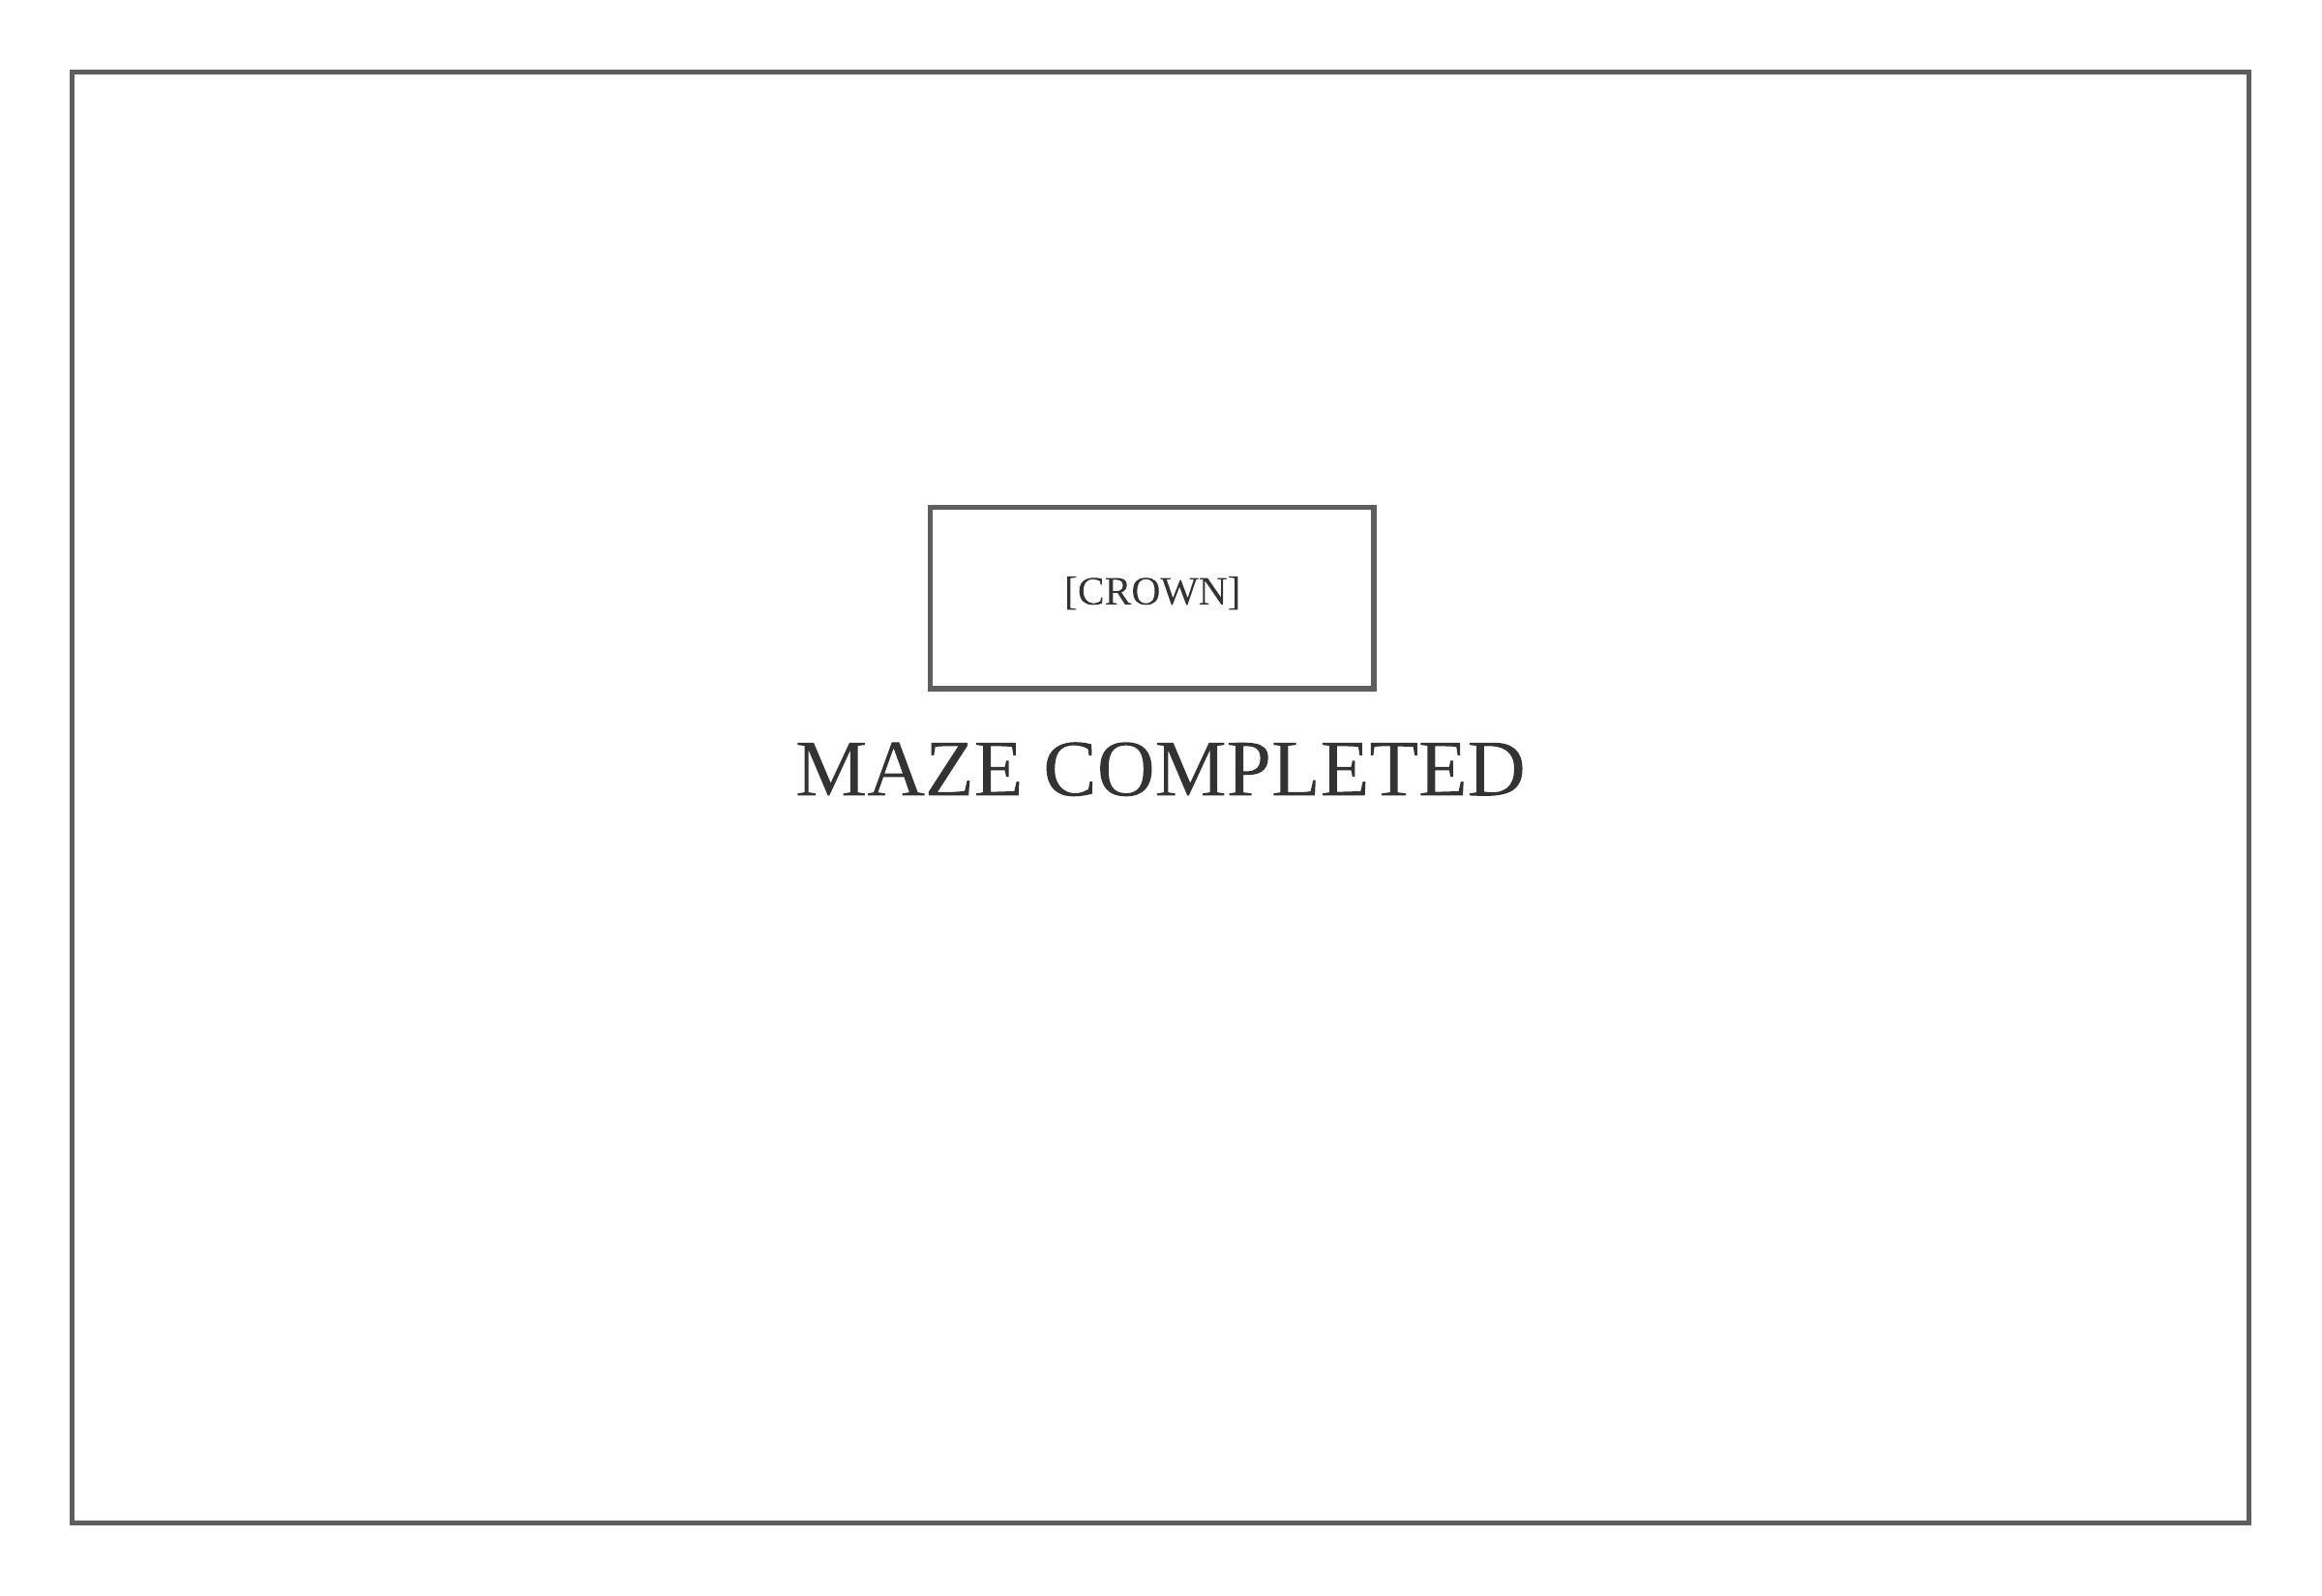
\includegraphics[scale=0.7]{Maze Completed}

	This screen is displayed for a few seconds after the maze is completed, it features the words "Maze Completed" along with a little pixel art crown.
\end{center}



%%%%%%%%%%%%%%%%%%%%%%%%%%
\clearpage
\part{Code Highlights}
\clearpage

%%%%%%%%%%%%%%%%%%%%%%%%%%
\clearpage
\part{Code breakdown by function}
\clearpage
\section{main.py}
This script handles the creation of the UI as well as running the Maze Database, MazeGenerationNew and 
MazeRendererNew scripts.

\textcolor[RGB]{220,220,220}{\rule{\linewidth}{0.2pt}}
\begin{lstlisting}
def change_state(state):      

    des()
    if state == "start":    
        title = tk.Label(window, text = "\n Maze Game \n Version 2.0 \n", bg = "white", borderwidth=1, relief="groove").pack(fill = "x",pady=(250,20))
        enter_button = tk.Button(window, text = "Enter",bg = "white",width=30, command = lambda: change_state("username")).pack()
        exit_button = tk.Button(window, text = "Exit",width=30, bg = "white", fg = "red", command = lambda: exit()).pack(pady=3)
        if not installed:
            error_message = tk.Label(window,text="[PIL not installed, PIL is required for current version]",fg="red").pack(side="bottom",pady = 20)
    if state == "username": 
        title = tk.Label(window, text = "\n Accounts \n", bg = "white",  borderwidth=1, relief="groove").pack(fill = "x",pady=(20,100))
        top_seperator = tk.Canvas(window, height=50,width=0).pack()
        ...
\end{lstlisting}
The "change state" function takes the argument "state" and uses that to switch to a pre-defined set of UI elements, e.g. a main menu or a user select screen.

\begin{lstlisting}
def create_levels(lower,upper,number_of_columns,title,maze_type,completed):
    des()
    first = tk.Frame(window)
    first.pack(side='top')
    side = first
    title_ = tk.Label(window, text = ("\n" + title + "\nSelect a level\n"), bg = "white", borderwidth = 1, relief = "groove").pack(in_ = first,fill = "x",pady=20)
    top_seperator = tk.Canvas(window, height=50,width=0).pack(in_ = side)
    dict_one = {
                "normal":0,
                "diamond":1
                }
    for i in range((lower),(upper+1)):
            text = str(i)                          
            try:
                if completed[dict_one[maze_type]].count(text) > 0:
                    fg = "green"
                    text += "\n(Complete)"
                else:
                    fg = "black"
            except:
                fg = "black"
            button = tk.Button(window, text=text, width = 10, relief = 'groove', bg = "white",fg = fg)
            button.config(command = lambda mt = maze_type, btn = button : load_maze(lower,upper,title,mt,dict_one[maze_type],btn))
            button.pack(in_ = side, side = "left", padx=10,pady=10)
            if (i%number_of_columns) == 0:
                middle = tk.Frame(window)
                middle.pack(side = "top")
                side = middle
    back_button = tk.Button(window, text = "Back", command = lambda: change_state("maze select")).pack(side="bottom",pady=10)

\end{lstlisting}
"Create levels" generates a set of buttons with numbers on them, defined by the range entered in the parameters (lower and upper). If the level has already been completed by the user then the text will be green! It lays them out based on the parameter "number\_of\_columns".
When the user clicks on one of these buttons the actual button is passed to the function so that the text on the button can be properly read.

\clearpage

\begin{lstlisting}
def load_maze(lower,upper,title,maze_type,btn):   #Generates the maze and then passes the data along with other parameters to the MazeRenderer script
    maze_size = int((btn['text']).replace("\n(Complete)","")) + 3
    if installed:        
        maze_data = main(maze_size,maze_size,1000,maze_type)
        dict_two = {
            "normal":[[len(maze_data[0])-1],[0],[0,len(maze_data)-1]],
            "diamond":[[len(maze_data[0])-1],[0],[0,len(maze_data)-1]]
            }
        win_pos_x = (dict_two[maze_type])[0]
        win_pos_y = (dict_two[maze_type])[1]
        start_pos = (dict_two[maze_type])[2]
        dimensions = alter_screen()
        won = play_maze(dimensions[0],dimensions[1],(str(maze_size) + " x " + str(maze_size)),10,win_pos_x,win_pos_y,start_pos,maze_data)
    else:
        won = True  #Maze auto-completes if PIL is not installed
    if won:
        if user_id != 0:
            Db.add_completed_level(connection,maze_size-3, maze_type,user_id)
    completed = Db.get_list_of_completed_levels(connection,user_id)
    create_levels(lower,upper,4,title,maze_type,completed)

\end{lstlisting}
The main job of "Load Maze" is to translate the parameters entered pass them to the MazeGenerationNew, script take the generated
data and then pass that, along with other translated parameters, to the MazeRenderNew script.

\begin{lstlisting}
def custom_maze(maze_type,width,height,cube_size,title):    #Same as the function above but for custom mazes
        width = int(width.get())
        height = int(height.get())
        cube_size = int(cube_size.get())
        maze_data = main(width,height,1000,maze_type.get())
        dimensions = alter_screen()
        play_maze(dimensions[0],dimensions[1],(str(width) + " x " + str(height)),cube_size,[len(maze_data[0])-1],[0],[0,len(maze_data)-1],maze_data)
        change_state('custom maze',True)

\end{lstlisting}
"Custom Maze" is a version of "Load Maze" for cutom mazes with unsual heights and widths. An improvement to the code would be combining the two above functions.

\begin{lstlisting}
def set_user_id(username,guest):    #Sets the user ID
    global user_id
    if guest:
        user_id = 0
    else:
        user_id = username
    change_state("maze select")

\end{lstlisting}
"Set User ID" is a simple function that sets the global user\_id. The user\_id is used to retrieve data about the user from maze.db, if the user is a guest then the ID is set to 0
and all code involving the user\_id is skipped.

\begin{lstlisting}
def reset_progress():           #Resets the current users progress
    username = Db.delete_user(connection, user_id)
    Db.create_new_user(connection, username)
    change_state("maze select")
\end{lstlisting}
This functions is also simple. It resets the progress of the user by deleting the user from the and then creating them again, utilizing the below function.

\begin{lstlisting}
def new_user(user_entry_widget):    #Creates a new user named using the entered user name
    name = user_entry_widget.get()
    Db.create_new_user(connection,name)
    change_state("username")
\end{lstlisting}
Simply, adds a new entry to the database containing a new user.

\clearpage

\begin{lstlisting}
def des(): #Deletes all current widgets in "window"
    widget_list = all_children(window)
    for item in widget_list:
        item.pack_forget()
\end{lstlisting}
This function deletes all current widgets, this is used to reset the UI so that new UI can be made in its place. It utilizes the below function
which creates a list of all widgets pareneted to the entered object. The object entered in the case of "des()"  is the whole tkinter window.
\begin{lstlisting}
def all_children(window): # This makes a list of all the current widgets
    list_one = window.winfo_children()
    for item in list_one:
        if item.winfo_children() :
            list_one.extend(item.winfo_children())
    return list_one
\end{lstlisting}

\begin{lstlisting}
def alter_screen():     #Changes screen dimenions to make the rendering of the maze faster
    const = 2
    dimensions = [0,0]
    dimensions[0] = int(screen_width/const)
    dimensions[1] = int(screen_height/const)
    return dimensions
\end{lstlisting}
"Alter Screen" shrinks the size of the layers (images created in the renderer) to make the creation of said layers in the rendering section of the code easier
and less resource consuming.

%%%%%%%%%%%%%%%%%%%%%%%%%%

\clearpage
\section{MazeDatabase.py}
Script for interaction with the maze.db for storing users and completed levels, utilizes SQL.

\textcolor[RGB]{220,220,220}{\rule{\linewidth}{0.2pt}}
\begin{lstlisting}
def main_database():    #Creates the database (if it wasn't already created) and establishes a connection to it 
    user_table = " CREATE TABLE IF NOT EXISTS users (
id integer PRIMARY KEY,
username text NOT NULL
); "
    completed_levels_table = " CREATE TABLE IF NOT EXISTS completedLevels (
id integer PRIMARY KEY,
normal_maze text,
diamond_maze text,
user_id integer NOT NULL,
FOREIGN KEY (user_id) REFERENCES users (id)
); " 
    connection = create_connection(r"Maze.db")
    if connection is not None:
        create_table(connection,user_table)
        create_table(connection,completed_levels_table)
    else:
        print("Database Connection Error")
    return connection
\end{lstlisting}
This function is run to intialize the database, composed of two tables, (if it's not already created) and  establish a connection to said database.
The comment explaining the datbase is included below, along with a diagram.
\begin{lstlisting}
"DATABASES
Users table stores name and user_id + any additional information needed
CompletedLevels table stores the completed levels linked to the foreign key user_id and a primary key completed_id. There will be two columns, one for normal mazes, one for diamond mazes
the completed levels will be serialized as such (1#3#4#12...) and when the string is imported it will be split into a list."
\end{lstlisting}
\begin{center}
	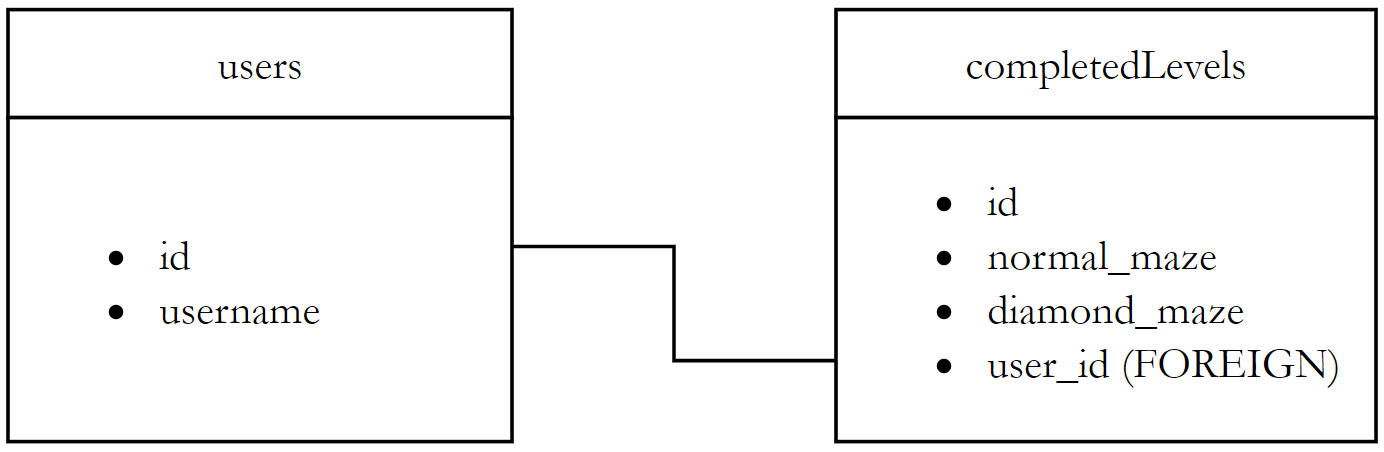
\includegraphics[scale=0.5]{Database Diagram}
\end{center}
\begin{lstlisting}
def create_new_user(connection, username):
    #Create the new user
    new_user_sql = "INSERT INTO users(username) VALUES(?)"
    cursor = connection.cursor()
    cursor.execute(new_user_sql, (username,))
    user_id = cursor.lastrowid
    connection.commit()
    #Then create the sibling entry in the CompletedLevels table based of the generated user_id
    new_completed_levels_sql = "INSERT INTO completedLevels(normal_maze, diamond_maze, user_id) VALUES(?,?,?)"
    cursor = connection.cursor()
    cursor.execute(new_completed_levels_sql, ("","",user_id))
    connection.commit()
\end{lstlisting}
"Create New User" inserts a row into the \textbf{users} table containing the entered username and then makes a sister entry in \textbf{completedLevels}. It uses
cursor.lastrowid to get the correct user id.
\clearpage
\begin{lstlisting}
def delete_user(connection, user_id):
    sql = 'SELECT username FROM users WHERE id = ?'
    cursor = connection.cursor()
    cursor.execute(sql, (user_id))
    result = cursor.fetchall()
    #Delete user entry
    sql = 'DELETE FROM users WHERE id=?'
    cursor = connection.cursor()
    cursor.execute(sql, (user_id))
    connection.commit()
    #Delete completedLevels entry
    sql = 'DELETE FROM completedLevels WHERE user_id=?'
    cursor = connection.cursor()
    cursor.execute(sql, (user_id))
    connection.commit()
    return result[0][0]
\end{lstlisting}
"Delete User" removes an entry from users and completedLevels based on the entered user\_id. It will also return the username from said user so that they can
be recreated in the "Reset Progress" function.

\begin{lstlisting}
def get_list_of_users(connection):
    user_list = []
    cursor = connection.cursor()
    cursor.execute("SELECT * FROM users")
    result = cursor.fetchall()
    for row in result:
        user_list.append((str(row)[1:-1]).split(','))
    return user_list
\end{lstlisting}
This function is implemented in "Change State" and is used when creating the buttons for the users in the user select screen. Contained within each
entry in the list is both the user\_id and the username.

\begin{lstlisting}
def add_completed_level(connection, level_number, maze_type, user_id):    #Uses the user id to alter the user's completed levels
    completed = get_list_of_completed_levels(connection, user_id)
    dict_one = {
                "normal":0,
                "diamond":1
                }
    formatted = ''
    for level_num in completed[dict_one[maze_type]]:
        print(level_num)
        formatted = formatted + level_num + "#"
    formatted = formatted + str(level_number)
    if maze_type == "normal":
        sql = "UPDATE completedLevels SET normal_maze = ? WHERE user_id = ?"
    elif maze_type == "diamond":
        sql = "UPDATE completedLevels SET diamond_maze = ? WHERE user_id = ?"
    cursor = connection.cursor()
    cursor.execute(sql,(formatted,user_id))
\end{lstlisting}
"Add Completed Level" takes the current completed levels list converts it to a string,  adds the entered level to the string and then inserts
it into the correct entry in the database. It finds the correct entry based off the maze type and user\_id.
\begin{lstlisting}
\end{lstlisting}
The below function is implemented in "Add Completed Level" to get the current completed levels for both maze types.
\begin{lstlisting}
def get_list_of_completed_levels(connection, user_id):
    maze_find_sql = "SELECT normal_maze, diamond_maze FROM completedLevels WHERE user_id = ?"
    cursor = connection.cursor()
    cursor.execute(maze_find_sql,(user_id))
    result = cursor.fetchall()
    return [(result[0][0]).split('#'),(result[0][1]).split('#')]
\end{lstlisting}
"Get List of Completed Levels" takes the string stored in the database for all maze types and converts them into a 2D array. 
The format for the string is explained in the comment explaning the database above.

\clearpage
\begin{lstlisting}
def create_connection(db_file):
    connection = None
    try:
        connection = sqlite3.connect(db_file)
    except Error as e:
        print(e)
    return connection
\end{lstlisting}

\begin{lstlisting}
def create_table(connection, create_table):
    try:
        cursor = connection.cursor()
        cursor.execute(create_table)
    except Error as e:
        print(e)
\end{lstlisting}
The above two functions are standard functions for interacting with a database. "Create Conncetion" creates a connection with a database file or creates the
database file and the establishes a connection with it if it doesn't already exist. The connection is then used the interact with the database itself. "Create Table"
actually would execute any SQL passed to it and acts more like an alias/simplification, however, it is only ever used to create tables.

%%%%%%%%%%%%%%%%%%%%%%%%%%

\clearpage
\section{MazeGenerationNew.py}
Uses Kruskal’s algorithm paired with a generated weight array to create the maze.

\textcolor[RGB]{220,220,220}{\rule{\linewidth}{0.2pt}}
\begin{lstlisting}
def intialize_array(width,height):
    #Intialize the array
    maze_array = []
    for x in range(0,width):
        maze_array.append([])
        for y in range(0,height):
            maze_array[x].append([1,1,1,1]) #Add a blank cell with all four walls to create an array that will be altered to generate a maze, this array is the data we return
    return maze_array
\end{lstlisting}
"Intialize Array" creates a 2D array formatted in the correct manner to be used as the \textbf{maze\_array} which represents the maze. This maze is made
up of cells, each cell being linked to a coordinate/index in the 2D array, with the cell being represented as a list of length four (i.e. [1,1,1,1]). Each number in
this list can be eithier a 1 or 0, representing a wall or empty space respectively. A diagram displaying this is placed below.
\begin{center}
	\fbox{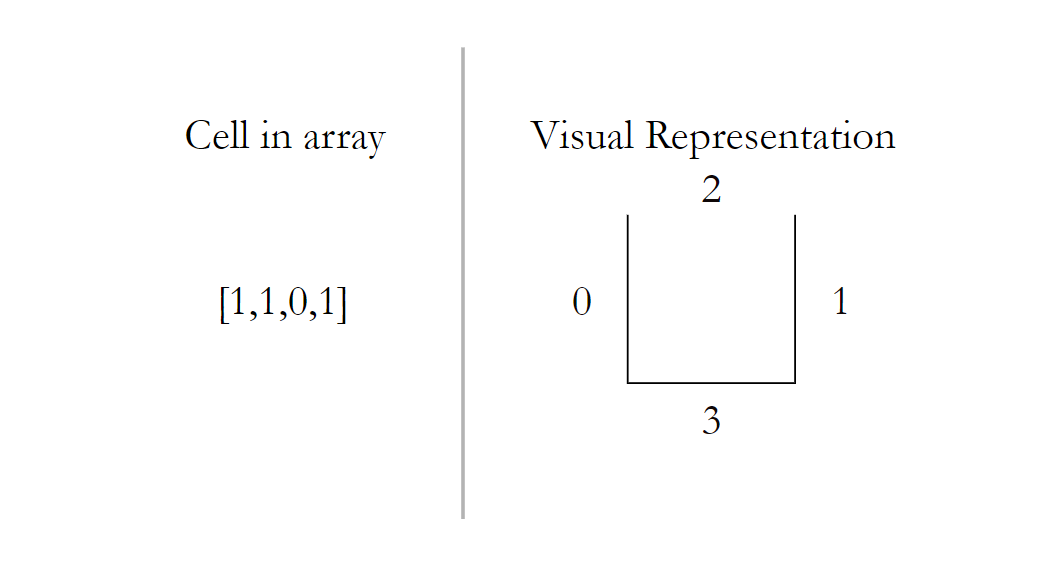
\includegraphics[scale=0.5]{Maze Cell Diagram}}

	\color{mygrey}(The numbers on the Visual Representation correlate to the index in the array)
\end{center}

\begin{lstlisting}
def generate_random_walls(height,width):    #Random walls for testing maze renderer
    #Intialize the array
    maze_array = []
    temp_list = [0,0,0,0,0,0,1]
    for x in range(0,width):
        maze_array.append([])
        for y in range(0,height):
            maze_array[x].append([random.choice(temp_list),random.choice(temp_list),random.choice(temp_list),random.choice(temp_list)])
    return maze_array
\end{lstlisting}
The above function is used only in testing, it can technically generate unbeatable mazes but due to the weighted chance to generate an empty or 
a wall (represented using temp\_list) it is unlikley. It  was mainly used in rendering testing but was also used when testing maze collision. 
\clearpage
\begin{lstlisting}
def kruskals_algorithim(weight_group_array,width,height,max_weight): #Based loosely on the algorithim as described in "Mazes for Programmers"
    maze_array = intialize_array(width,height)
    group_designation = 1                                                                                                                                           
    temp_list_empty = False
    while not all_in_one_group(weight_group_array,height,width) and not temp_list_empty: #Only ends loop when no new corridors can be checked and all the corriders are in the same group
        temp_list = lowest_values_pos(weight_group_array,width,height,max_weight+1)
        if temp_list == []:
            temp_list_empty = True
        else:
            dict_one = {
                0:[0,-1,1],
                1:[0,1,0],
                2:[-1,0,3],
                3:[1,0,2]
                }
            for pos in temp_list:
                can_connect = True
                difference = dict_one[pos[2]]
                current_pos_group = (weight_group_array[pos[0]][pos[1]])[4]                
                try:
                    if pos[0]+difference[0] == -1 or pos[1]+difference[1] == -1:
                        error = pos[100]
                    connected_pos_group = (weight_group_array[pos[0]+difference[0]][pos[1]+difference[1]])[4]
                    if current_pos_group == 0:
                        if connected_pos_group == 0:
                            (weight_group_array[pos[0]][pos[1]])[4] = group_designation
                            (weight_group_array[pos[0]+difference[0]][pos[1]+difference[1]])[4] = group_designation
                            group_designation += 1
                        else:
                            (weight_group_array[pos[0]][pos[1]])[4] = (weight_group_array[pos[0]+difference[0]][pos[1]+difference[1]])[4]
                    else:
                        if current_pos_group == connected_pos_group:
                            can_connect = False
                        elif connected_pos_group == 0:
                            (weight_group_array[pos[0]+difference[0]][pos[1]+difference[1]])[4] = current_pos_group
                        elif connected_pos_group != 0:
                            group_pos = get_all_in_group(weight_group_array,width,height,connected_pos_group)
                            for pos2 in group_pos:
                                (weight_group_array[pos2[0]][pos2[1]])[4] = current_pos_group
                    if(can_connect):
                        (maze_array[pos[0]][pos[1]])[pos[2]] = 0
                        (maze_array[pos[0]+difference[0]][pos[1]+difference[1]])[difference[2]] = 0
                    (weight_group_array[pos[0]][pos[1]])[pos[2]] = max_weight+2
                    (weight_group_array[pos[0]+difference[0]][pos[1]+difference[1]])[difference[2]] = max_weight+2
                except IndexError:
                    (weight_group_array[pos[0]][pos[1]])[pos[2]] = max_weight+2
                    if (weight_group_array[pos[0]][pos[1]])[4] == 0:
                        (weight_group_array[pos[0]][pos[1]])[4] = group_designation
                        group_designation += 1
    return maze_array
\end{lstlisting}
"Kruskals Algorithim" is the algorithim used to actually generate the mazes. It does this utilizing a \textbf{weight\_group\_array} and by altering
the corridors between cells in the \textbf{maze\_array}. The outline of how it works is this; All cells have a group, at the start this is the default group (i.e. zero).
Any cell within a group is reachable by any other cell in a group (unless it is the default group), they are essentially perfect mazes within the larger maze.
At the start of each iteration of the while loop the code finds corridors (connections between cells) based on the lowest weight, this is done using the afformentioned
\textbf{weight\_group\_array} and the function below.
\clearpage
\begin{lstlisting}
def lowest_values_pos(wg_array,width,height,compared_to):   #Finds all the connections in the maze with the lowest weight value
    temp_list = []
    for x in range(0,width):
        for y in range(0,height):
            for i in range(0,4):
                if wg_array[x][y][i] < compared_to:
                    compared_to = wg_array[x][y][i]
                    temp_list = []
                    temp_list.append([x,y,i])
                elif wg_array[x][y][i] == compared_to:
                    temp_list.append([x,y,i])
    return temp_list
\end{lstlisting}
The actual \textbf{weight\_group\_array} or\textbf{wg\_array}  is generated by functions "Generate Walled Maze" and "Generate Diamond Maze" discussed lower down.
Once a corridor is chosen an actual connection is attempted, a connection will only not be made if, 1. The connection is being made to an area outside the maze or 2. The
connection is being made to a cell that is already in the same group as the chosen cell. The latter of the two fail states exists so that the generation doesn't remove every single wall.
If a connection is made between two cells with non-default but different groups then all cells in the group that doesn't contain the chosen cell are changed to be in the group
with the chosen cell. This process is done using "Get All In Group" (shown below).
\begin{lstlisting}
def get_all_in_group(wg_array,width,height,group):  #Gets the positions of all the cells that have the group specified
    temp_array = []
    for x in range(0,width):
        for y in range(0,height):
            if (wg_array[x][y])[4] == group:
                temp_array.append([x,y])
    return temp_array
\end{lstlisting}
The algorithim will run untill all cells are in the same group (and that group is not the default) meaning any cell within the maze can be reached from any other cell. To check
that all cells are in the same group the function "All In One Group" is used.
\begin{lstlisting}
def all_in_one_group(wg_array,height,width):    #Checks to see if every cell is in a singular group (a.k.a every cell can be reached from any other cell)
    returned = True
    first_group = "null"
    for x in range(0,width):
        for y in range(0,height):
            temp = (wg_array[x][y])[4]
            if first_group == "null":
                first_group = temp
            if temp != first_group or temp == 0:
                returned = False                
    return returned
\end{lstlisting}
\begin{lstlisting}
def generate_walled_maze(width,height,max_weight):
    weight_group_array = []                 
    for x in range(0,width):
        weight_group_array.append([])
        for y in range(0,height):
            weight_group_array[x].append([random.randint(1,max_weight),random.randint(1,max_weight),random.randint(1,max_weight),random.randint(1,max_weight),0])   #Create a "sister" array that stores the weight values and group of each cell
    maze_array = kruskals_algorithim(weight_group_array,width,height,max_weight)    #Use the weight array to generate an actual maze
    return maze_array
\end{lstlisting}
"Generate Walled Maze" generates a simple \textbf{weight\_group\_array} by randomly generating weight values for each cell.
\clearpage
\begin{lstlisting}
def generate_diamond_maze(width,height,max_weight):
    weight_group_array = []
    for x in range(0,width):
        weight_group_array.append([])
        for y in range(0,height):
            weight_group_array[x].append([random.randint(1,max_weight),random.randint(1,max_weight),random.randint(1,max_weight),random.randint(1,max_weight),0])
    #Manipulate the weight group array to make the algorithim generate a diamond maze with random gaps in the walls
    center_of_maze = [int(width/2),int(height/2)]
    pos_to_change = center_of_maze
    counter = 1
    circling = True
    translate_to_displacement = {
        1:[0,1],
        2:[1,0],
        3:[0,-1],
        0:[-1,0]
        }
    translate_to_wall_index = {
        1:2,
        2:1,
        3:3,
        0:0
        }
    while circling:
        modded_counter = counter % 4
        displacement = translate_to_displacement[modded_counter]
        wall_index = int(translate_to_wall_index[modded_counter])
        length_counter = counter // 2 + (counter % 2)
        for i in range(1,length_counter):
            #Check to see if current cell is within maze
            if pos_to_change[0] > width-1 or pos_to_change[1] > height-1:
                pass
            else:
                #If it is then remove the wall leading to the new cell
                weight_group_array[pos_to_change[0]][pos_to_change[1]][wall_index] = counter
            #Move into the new cell
            pos_to_change = [pos_to_change[0]+displacement[0],pos_to_change[1]+displacement[1]]
        counter += 1
        #Fail state check
        if pos_to_change[0] > width and pos_to_change[1] > height:
            circling = False
    weight_group_array[center_of_maze[0]][center_of_maze[1]] = [0,0,0,0,0] #Remove all walls from center
    maze_array = kruskals_algorithim(weight_group_array,width,height,max_weight)
    return maze_array 
\end{lstlisting}
"Generate Diamond Maze" is a more complicated  \textbf{weight\_group\_array} generator used to create a maze with an actual texture. It does this by
circling from cells from the maze center changing the weights so that the corridors are created in a certain way leading to a pyramid/diamond pattern. This method
could also be used to create a circular maze, however, that type of maze is significatly less fun to play. 

%%%%%%%%%%%%%%%%%%%%%%%%%%

\clearpage
\section{Window.py}
Uses tkinter, NumPy and pillow (a fork of PIL (Python Imaging Library)) to create layered editable images on screen. Using tkinter it also handles input, unfortunately the window needs to be clicked on for input to be registered.

\textcolor[RGB]{220,220,220}{\rule{\linewidth}{0.2pt}}
\begin{lstlisting}
class Window():
    pixel_scale = 1
    last_key_pressed = None
    
    def __init__(self, height, width, default_colour, title):   #Creates the intial image and sets intial values
        self.height = int(height)
        self.width = int(width)
        self.title = title
        self.default_colour = default_colour
        self.window = create_tkinter_window(self.height, self.width, self.title)
        self.screen = create_canvas(self.window)
        self.layers = []
        self.layers.append(self.Layer(self,self.height,self.width,self.default_colour)) #Create the background layer
\end{lstlisting}
Above is the "Window" class and its "\_\_init\_\_" function. A "Window" instance has a tkinter window (with a canvas called .screen) upon which
layers can be placed. In the "\_\_init\_\_" function only a background/default layer is created. Each layer is also an instance of
a class called "Layer", which is a sub-class of "Window". However, it being a sub-class doesn't actually mean anything (other than making it easier to
understand what "Layer" is meant for) so .layers is needed in "Window" to store that given window's layers. The code for "Layer" is shown below:
\begin{lstlisting}
    class Layer():  #Layer Objects

        def __init__(self,window,height,width,default_colour):
            self.height = height
            self.width = width
            self.default_colour = default_colour
            self.layer_num = len(window.layers)
            self.array = create_image_array(height,width,default_colour)
            self.generated_image = ImageTk.PhotoImage(master = window.screen,image=Image.fromarray(self.array))
            self.image = window.screen.create_image(width,height,image=self.generated_image)
\end{lstlisting}
Layers are used as a form of optimisation so that when we update the screen, to move the player for example, we only need
to update a very small image rather than the whole maze image. 
\begin{lstlisting}
    def move_layer(self,new_coords,layer_num = 0):  #Moves a layer to a given position
        #Get Current Top Left of layer Coords
        old_coords = self.screen.coords(self.layers[layer_num].image)
        old_coords[0] = old_coords[0] - (self.layers[layer_num].height/2)
        old_coords[1] = old_coords[1] - (self.layers[layer_num].width/2)
        #Move to new position
        self.screen.move(self.layers[layer_num].image,new_coords[0] - old_coords[0],new_coords[1] - old_coords[1])
\end{lstlisting}
"Move Layer" is moves any given layer to entered coordinates. While there is a standard move function for image objects on
tkinter canvases, it moves objects by a 2D Vector rather than being coordinate based.
\begin{lstlisting}
    def delete_layer(self,layer):
        self.screen.delete(self.layers[layer].image)
        self.layers.pop(layer) 
\end{lstlisting}
"Delete Layer" deletes a layer by first removing its image from the canvas and then poping it from the .layers list. Unlike other functions
that interact with layers this one requires a layer number to be entered (whereas others have a default of the background layer) so that
the background layer isn't deleted by mistake. 
\begin{lstlisting}
    def reset(self, layer_num = 0):    #Resets the entered layer, used so the line below doesn't need to be typed everytime
        self.layers[layer_num].array = create_image_array(self.layers[layer_num].height,self.layers[layer_num].width,self.layers[layer_num].default_colour)
\end{lstlisting}
There is also "Reset" which will just reset a layer (based of the "Window" object .default\_colour) rather than deleting it.
\begin{lstlisting}
    def set_pixel(self, coords, colour, layer_num=0): #Change a pixel in the image array
        coords[0] = (coords[0] * self.pixel_scale) - (self.pixel_scale - 1)
        coords[1] = (coords[1] * self.pixel_scale) - (self.pixel_scale - 1)
        for x in range(coords[0],coords[0]+self.pixel_scale):
            for y in range(coords[1],coords[1]+self.pixel_scale):
                try:
                    self.layers[layer_num].array[y,x] = colour
                except IndexError:
                    pass   
\end{lstlisting}
"Set Pixel" allows any pixel on the entered layer to be altered based off the coordinates entered, a range of pixels can also be affected 
if the pixel scale isn't one. It does this by altering the coresponding index in a numpy array, this numpy array is then converted into an
image using Pillow (PIL) and then subsequently turned into an image tkinter will accept, also using PIL. The image conversion is all done
in the "Update" function, alongside updating the tkinter window itself.
\begin{lstlisting}
    def update(self, layer_num = 0):   #Updates an entered layer
        try:
            self.layers[layer_num].generated_image = ImageTk.PhotoImage(master = self.screen,image=Image.fromarray(self.layers[layer_num].array)) #Generate a updated image from the image array
            self.screen.itemconfig(self.layers[layer_num].image, image = self.layers[layer_num].generated_image)    #Applies the generated image
        except IndexError:
            print("Invalid Layer")
        self.window.update()
\end{lstlisting}
\begin{lstlisting}
    def init_input(self):                   #Input created using tkinter, last key pressed = key pressed that frame
        def on_key_press(event):
            self.last_key_pressed = event.char
            if self.last_key_pressed == '\boxempty':
                self.last_key_pressed = 'esc'
        def on_key_up(event):
            self.last_key_pressed = None
        self.window.bind('<KeyPress>', on_key_press)
        self.window.bind('<KeyRelease>', on_key_up)
\end{lstlisting}
The "Window" class also handles input, utilizing tkinter's event system. "Init Input" must be run to start input and within the function two other
functions are also defined. "On Key Press" sets .last\_key\_pressed to the current key being pressed when a key is being pressed (as indicated by tkinter), while
"On Key Up" sets .last\_key\_pressed back to \textcolor{amber}{None}. 
\begin{lstlisting}
    def set_fullscreen(self, boolean):  #Turns fullscreen on and off based on boolean
        self.window.overrideredirect(True)
        self.window.overrideredirect(False)
        self.window.attributes('-fullscreen',boolean)
        self.screen.pack(fill="both", expand=True)

    def set_pixel_scale(self, num): #Used to change the pixel scale
        self.pixel_scale = num

    def quit(self):                             #Quits window
        for i in range(0,len(self.layers)):
            self.reset(i)
        self.window.destroy()
        del self
\end{lstlisting}
"Set Fullscreen", "Set Pixel Scale" and "Quit" are the three functions in the "Window" class that don't directly interact with a certain layer. "Set Fullscreen" allows for fullscreen
to be toggled on and off based on the parameter "boolean", "Set Pixel Scale" allows for the pixel scale to be changed in a less akward manner and "Quit" simply deletes every layer,
destroys the tkinter window and then does the same to the instance of the class.

\begin{lstlisting}
def create_tkinter_window(height, width, title):    #Creates a tkinter window
    window = tk.Tk()
    window.title(title)
    window.geometry(str(width) + "x" + str(height))
    #window.overrideredirect(1) #Removes the Titlebar
    return window
\end{lstlisting}
"Create Tkinter Window" and the two other final functions in "Window.py" aren't directly related to the "Window" class but are used within it. "Create Tkinter Window" simply creates
a tkinter window based of the parameters entered and then returns said window.
\begin{lstlisting}
def create_canvas(tkinter_window):  #Creates a tkinter canvas
    canvas = tk.Canvas(tkinter_window, bg="black")
    canvas.pack(fill="both",expand=True)
    return canvas
\end{lstlisting}
"Create Canvas" adds a canvas object to the passed tkinter window, the canvas is then made to fill the entire window. The canvas object it also returned.
\begin{lstlisting}
def create_image_array(height,width,colour): #Creates the intial image array
    image_array = np.zeros([height+1,width+1,3],dtype=np.uint8)
    image_array.fill(colour)
    return image_array
\end{lstlisting}
"Create Image Array" makes a numpy array and then fills it with the desired greyscale colour, entered as any value between 0 and 255, finnally the new image
array is returned.
%%%%%%%%%%%%%%%%%%%%%%%%%%

\clearpage
\section{MazeRendererNew.py}
Used when actually playing a maze, mainly used to implement the Window.py script to correctly draw the maze but also handles collision detection and a check to see if the player has won.

\textcolor[RGB]{220,220,220}{\rule{\linewidth}{0.2pt}}
\begin{lstlisting}
\end{lstlisting}
"Play Maze" is the longest function in my entire NEA totaling around 130 lines of code, hence I'll explain it section by section rather than all at once.
\begin{lstlisting}
def play_maze(width,height,title,cube_size,win_pos_x,win_pos_y,start_pos,maze_data):
    #A cube_size of two and below will cause the squares to be too small to be properly represented properly on any pixelated screen, hence, 3 is the lowest the function allows
    if cube_size < 3: cube_size = 3 
    screen = Window.Window(height,width,0,"Test Window")
    screen.set_fullscreen(True)
    screen.init_input()
    screen.update()
    temp = 0 #Temporary Variable to manage progress of stand-in progress bar
    delta_time = 0
    fps = 0
    time_to_close = 1.5
    add_to_y = 0
    add_to_x = 0
    loading = True
    first_frame = True
    running = True
    position_set_to = [1,0]
    move_dir = ""
    player_pos = start_pos
    active_last_frame = True
    check_walls = True
    to_return = False
    ending = True
    drawing_per_frame = False
    input_confirmed = False
    input_delay = 0
\end{lstlisting}


%%%%%%%%%%%%%%%%%%%%%%%%%%

\clearpage
\section{Required Libraries}
To install all required packages the following commands must be run in command line                      
\begin{lstlisting}
python -m pip install --upgrade pip
python -m pip install --upgrade Pillow
python -m pip install --upgrade numpy
\end{lstlisting}
Pillow Website: \url{https://pillow.readthedocs.io/en/stable/installation.html}

\end{document}